% Reporte del Proyecto Final - Modelos Estadísticos
% Compilar con XeLaTeX desde la carpeta reporte/:  latexmk -xelatex reporte.tex
\documentclass[10pt,letterpaper,twocolumn]{article}

% ---- Idioma, tipografía y página ----
\usepackage[spanish,es-nodecimaldot,es-tabla,es-noshorthands]{babel}
\usepackage{fontspec}
\setmainfont{Literata}[
  Path           = fonts/,
  Extension      = .ttf,
  UprightFont    = *-Regular,
  BoldFont       = *-Bold,
  ItalicFont     = *-Italic,
  BoldItalicFont = *-BoldItalic]
\setmonofont{Consolas}[Scale = MatchLowercase]

\usepackage[top=2cm, bottom=2.2cm, left=1.8cm, right=1.8cm, columnsep=0.75cm]{geometry}
\usepackage{graphicx}
\graphicspath{{../plots/}}
\usepackage{booktabs}
\usepackage{placeins}
\usepackage{tabularx}
\usepackage{array}
\usepackage{enumitem}
\setlist{nosep, leftmargin=1.3em}
\usepackage{titlesec}
\usepackage[labelfont=bf, labelsep=period, font=small, skip=5pt]{caption}
\usepackage{listings}
\usepackage[hidelinks]{hyperref}

\setlength{\parindent}{0pt}
\setlength{\parskip}{4pt}
\renewcommand{\arraystretch}{1.08}

% ---- Colocación de figuras y tablas ----
\renewcommand{\topfraction}{0.85}
\renewcommand{\bottomfraction}{0.6}
\renewcommand{\textfraction}{0.1}
\renewcommand{\floatpagefraction}{0.8}
\renewcommand{\dbltopfraction}{0.85}
\renewcommand{\dblfloatpagefraction}{0.8}

% ---- Encabezados de sección (la numeración sigue la del script de R) ----
\setcounter{secnumdepth}{0}
\titleformat{\section}{\large\bfseries}{}{0pt}{}
\titlespacing*{\section}{0pt}{12pt}{4pt}
\titleformat{\subsection}{\normalsize\bfseries}{}{0pt}{}
\titlespacing*{\subsection}{0pt}{9pt}{3pt}

% ---- Fragmentos de código R: solo negro, negritas e itálicas ----
\lstdefinelanguage{Rsimple}{
  keywords   = {function, if, else, for, in, TRUE, FALSE, NA, NULL},
  sensitive  = true,
  morecomment = [l]{\#},
  morestring  = [b]",
}
\lstset{
  language          = Rsimple,
  basicstyle        = \ttfamily\fontsize{7.3}{8.9}\selectfont,
  keywordstyle      = \bfseries,
  commentstyle      = \itshape,
  stringstyle       = \upshape,
  numbers           = left,
  numberstyle       = \ttfamily\fontsize{6}{8}\selectfont,
  numbersep         = 5pt,
  xleftmargin       = 1.6em,
  framexleftmargin  = 1.6em,
  frame             = lines,
  framerule         = 0.4pt,
  breaklines        = true,
  breakatwhitespace = true,
  postbreak         = \mbox{\ensuremath{\hookrightarrow}\space},
  columns           = fullflexible,
  keepspaces        = true,
  showstringspaces  = false,
  extendedchars     = true,
  aboveskip         = 6pt,
  belowskip         = 4pt,
}

% ---- Atajos ----
\newcommand{\var}[1]{\texttt{#1}}
\newcommand{\Hcero}{\textit{H}\textsubscript{0}}
\newcommand{\etaH}{η²\textsubscript{\textit{H}}}
\newcommand{\pval}{\textit{p}}
\newcommand{\sci}[2]{#1\,×\,10\textsuperscript{−#2}}

\begin{document}

% ---- Inicio a una columna ----
\twocolumn[{%
  \begin{center}
    {\LARGE\bfseries Proyecto Final: Modelos Estadísticos\par}
    \vspace{5pt}
    {\large\itshape Análisis estadístico de la base de datos \textup{\var{Wine.csv}}\par}
    \vspace{14pt}
    {\large\bfseries Alexis Alberto Zúñiga Alonso\par}
    \vspace{2pt}
    {\large\bfseries Baruc Azael Ramírez Romo\par}
    \vspace{10pt}
    Profesor: Axel Torres\par
    \vspace{2pt}
    \textit{EdgeHub | School of Innovation}\par
    \vspace{2pt}
    9 de octubre de 2026\par
  \end{center}
  \vspace{6pt}
  \hrule
  \vspace{16pt}
}]

% =======================================================================
\section{Descripción}

La base de datos \var{Wine.csv} contiene 178 muestras de vino y 14 variables. Trece de ellas son mediciones químicas de cada muestra y la variable \var{Customer\_Segment} se interpreta como el \textbf{pueblo} donde se extrajo el vino (1, 2 o 3). La variable \var{Proline} se define como la concentración de prolina en mg/L.

El trabajo sigue los tres apartados del script de R: (1)~limpieza de datos, (2)~análisis exploratorio y (3)~inferencia estadística y modelos. Cada fragmento de código se acompaña de una descripción del procedimiento y de los resultados numéricos que produjo.

% =======================================================================
\section{0. Preparación del entorno}

\begin{lstlisting}[firstnumber=41]
# Instala (si faltan) y carga los paquetes; MASS y nnet se llaman con `::` para no enmascarar dplyr::select
libs <- c("tidyverse", "car", "rstatix", "ggpubr", "caret", "patchwork")
faltantes <- libs[!libs %in% rownames(installed.packages())]
if (length(faltantes) > 0) install.packages(c(faltantes, "MASS", "nnet"))
invisible(lapply(libs, library, character.only = TRUE))
\end{lstlisting}

Se cargan los paquetes utilizados: \var{tidyverse} (manipulación de datos y gráficas), \var{car} (prueba de Levene, VIF y Breusch-Pagan), \var{rstatix} (pruebas de hipótesis y tamaños de efecto), \var{ggpubr} y \var{patchwork} (anotación y composición de gráficas), \var{caret} (partición de datos, validación cruzada y métricas), \var{MASS} (selección de variables por AIC) y \var{nnet} (regresión logística multinomial). El análisis se ejecutó en R~4.6.1.

% =======================================================================
\section{1. Limpieza de datos}

\subsection{1.a Comprensión de las variables y sus registros}

\begin{lstlisting}[firstnumber=71]
# Carga de datos crudos y vistazo a la estructura (178 muestras x 14 variables)
wine_raw <- read_csv("data/Wine.csv", show_col_types = FALSE)
glimpse(wine_raw)
\end{lstlisting}

Se leen los datos crudos y \var{glimpse()} muestra su estructura: 178 filas, 14 columnas, todas leídas por R como numéricas. Con base en ello se construyó un diccionario de datos con la descripción, unidad propuesta y tipo estadístico de cada variable (Tabla~\ref{tab:diccionario}).

\begin{table}[htbp]
  \centering
  \caption{Diccionario de datos.}
  \label{tab:diccionario}
  \footnotesize
  \begin{tabularx}{\columnwidth}{@{}l>{\raggedright\arraybackslash}Xl@{}}
    \toprule
    \textbf{Variable} & \textbf{Descripción} & \textbf{Unidad} \\
    \midrule
    \var{Alcohol}              & Contenido de alcohol         & \% vol \\
    \var{Malic\_Acid}          & Ácido málico                 & g/L \\
    \var{Ash}                  & Cenizas (residuo mineral)    & g/L \\
    \var{Ash\_Alcanity}        & Alcalinidad de las cenizas   & meq/L \\
    \var{Magnesium}\textsuperscript{d}      & Magnesio                     & mg/L \\
    \var{Total\_Phenols}       & Fenoles totales              & g/L \\
    \var{Flavanoids}           & Flavonoides                  & g/L \\
    \var{Nonflavanoid\_Phenols}& Fenoles no flavonoides       & g/L \\
    \var{Proanthocyanins}      & Proantocianidinas (taninos)  & g/L \\
    \var{Color\_Intensity}     & Intensidad de color          & absorb. \\
    \var{Hue}                  & Tonalidad del color          & razón \\
    \var{OD280}                & Razón OD280/OD315            & razón \\
    \var{Proline}\textsuperscript{d}        & Concentración de prolina     & mg/L \\
    \var{Customer\_Segment}\textsuperscript{n} & Pueblo de origen (1, 2, 3) & --- \\
    \bottomrule
  \end{tabularx}
  \par\smallskip
  \raggedright\scriptsize Todas son cuantitativas continuas, salvo \textsuperscript{d}cuantitativa discreta y \textsuperscript{n}cualitativa nominal.
\end{table}

\begin{lstlisting}[firstnumber=95]
# Clase con la que R leyó cada variable y número de valores distintos (Customer_Segment solo tiene 3)
tibble(Variable = names(wine_raw),
       Clase_R  = map_chr(wine_raw, class),
       Valores_distintos = map_int(wine_raw, n_distinct))

# Número de muestras por pueblo (clases moderadamente desbalanceadas: 59, 71 y 48)
count(wine_raw, Customer_Segment)
\end{lstlisting}

Contar los valores distintos permite distinguir el tipo de variable: \var{Customer\_Segment} solo toma 3 valores, por lo que es \textit{cualitativa nominal} aunque R la lea como número; el resto toma entre 39 y 133 valores distintos. El conteo por pueblo da 59, 71 y 48 muestras (Figura~\ref{fig:muestras}).

\begin{figure}[htbp]
  \centering
  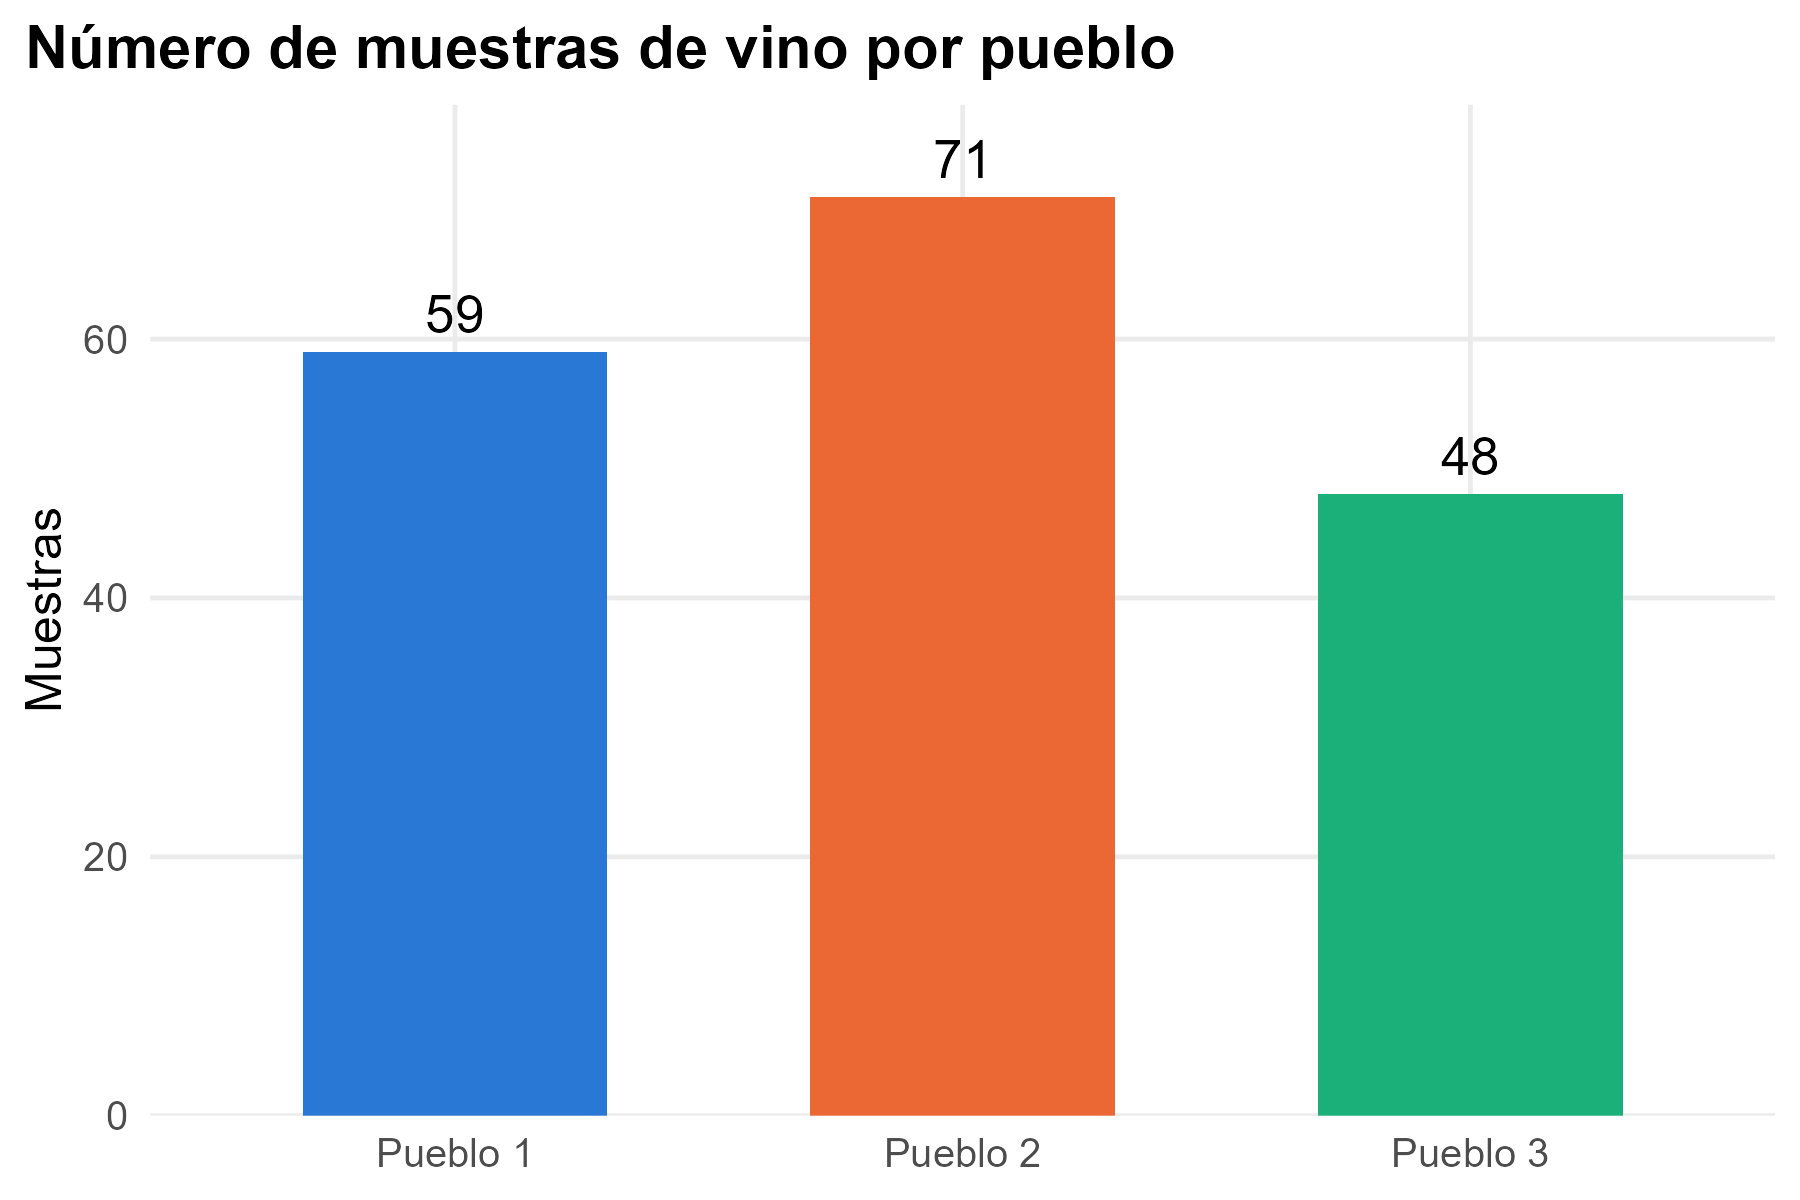
\includegraphics[width=0.92\columnwidth]{01_muestras_por_pueblo.png}
  \caption{Número de muestras de vino en cada pueblo: 59 en el Pueblo~1, 71 en el Pueblo~2 y 48 en el Pueblo~3.}
  \label{fig:muestras}
\end{figure}

\subsection{1.b Enfoque del análisis}

El enfoque es \textbf{mixto}: \textit{exploratorio} en la sección~2, para describir las variables, e \textit{inferencial y predictivo} en la sección~3, para comparar los pueblos, modelar la prolina y clasificar el pueblo de origen.

\subsection{1.c Detección de NAs, duplicados y valores anómalos}

\begin{lstlisting}[firstnumber=120]
# Conteo de NAs por variable
colSums(is.na(wine_raw))

# Filas completamente duplicadas
sum(duplicated(wine_raw))

# Valores negativos (imposibles en concentraciones químicas)
colSums(wine_raw < 0, na.rm = TRUE)

# Valores con más de 3 decimales: artefactos de formato (p. ej. Color_Intensity = 9.899999)
wine_raw %>%
  mutate(fila = row_number()) %>%
  pivot_longer(-fila, names_to = "Variable", values_to = "Valor") %>%
  filter(abs(Valor * 1000 - round(Valor * 1000)) > 1e-6)
\end{lstlisting}

Se revisan cuatro problemas posibles. Resultados: \textbf{0} valores faltantes (NA) en todas las variables, \textbf{0} filas duplicadas y \textbf{0} valores negativos. Se encontró \textbf{1} valor con más de tres decimales (fila 172, \var{Color\_Intensity} = 9.899999), atribuible a un error de formato.

\subsection{1.d Tratamiento de los casos detectados}

\begin{lstlisting}[firstnumber=137]
# Pipeline de limpieza: aplica cada paso solo si el problema existe, así sirve para futuras versiones del CSV
wine <- wine_raw %>%
  mutate(across(everything(), ~ round(.x, 3))) %>%  # elimina artefactos de redondeo
  filter(!is.na(Customer_Segment)) %>%  # sin pueblo no se puede imputar
  mutate(Pueblo = factor(Customer_Segment, levels = 1:3, labels = names(colores_pueblo))) %>%
  select(-Customer_Segment) %>%
  group_by(Pueblo) %>%
  mutate(across(where(is.numeric), ~ replace_na(.x, median(.x, na.rm = TRUE)))) %>%  # NA -> mediana del pueblo
  ungroup() %>%
  mutate(across(c(Magnesium, Proline), as.integer)) %>%  # variables de conteo a entero
  distinct()  # elimina filas duplicadas

# Verificación: sin NAs ni duplicados y mismas dimensiones que el original
stopifnot(sum(is.na(wine)) == 0, !any(duplicated(wine)))
dim(wine)
\end{lstlisting}

La limpieza se realiza en una sola cadena de pasos:
\begin{enumerate}
  \item Redondeo a 3 decimales para corregir el valor 9.899999.
  \item Eliminación de filas sin pueblo, ya que esa variable no se puede imputar.
  \item Conversión del pueblo a \textit{factor} (variable categórica).
  \item Imputación de NAs con la \textbf{mediana de su pueblo}. Se elige la mediana porque, a diferencia de la media, no se ve afectada por valores atípicos.
  \item Conversión de \var{Magnesium} y \var{Proline} a enteros.
  \item Eliminación de filas duplicadas.
\end{enumerate}
Como no hubo NAs ni duplicados, los pasos 2, 4 y 6 no modificaron los datos, pero quedan listos por si cambia el archivo. La verificación final confirma una base limpia de \textbf{178 × 14}, que se exporta como \var{Wine\_clean.csv}.

% =======================================================================
\section{2. Análisis Exploratorio de Datos}

\subsection{2.1 Medidas de tendencia central y dispersión}

\begin{lstlisting}[firstnumber=180]
tabla_descriptiva <- datos_largos %>%
  group_by(Variable) %>%
  summarise(
    N = n(),
    Media = mean(Valor),
    Mediana = median(Valor),
    Desviacion_estandar = sd(Valor),
    Varianza = var(Valor),
    Minimo = min(Valor),
    Primer_cuartil = quantile(Valor, 0.25),
    Tercer_cuartil = quantile(Valor, 0.75),
    Maximo = max(Valor),
    IQR = IQR(Valor),
    Rango = max(Valor) - min(Valor),
    Coeficiente_variacion = 100 * sd(Valor) / mean(Valor),
    .groups = "drop"
  ) %>%
  arrange(Variable)
\end{lstlisting}

Para cada variable se calculan medidas de \textbf{tendencia central} (media y mediana) y de \textbf{dispersión}: desviación estándar, varianza, rango y rango intercuartílico (IQR = Q3 − Q1, el ancho del 50\,\% central de los datos). El \textbf{coeficiente de variación} (CV = 100 · \textit{s} / \textit{x̄}) expresa la dispersión como porcentaje de la media, lo que permite comparar variables con unidades distintas (Tabla~\ref{tab:descriptiva}). Con el mismo código agrupado por pueblo se obtuvo la tabla \var{tabla\_descriptiva\_por\_pueblo.csv}.

\begin{table}[htbp]
  \centering
  \caption{Estadísticas descriptivas (\textit{n} = 178).}
  \label{tab:descriptiva}
  \footnotesize
  \setlength{\tabcolsep}{3.5pt}
  \begin{tabular}{@{}lrrrrr@{}}
    \toprule
    \textbf{Variable} & \textbf{Media} & \textbf{Mediana} & \textbf{DE} & \textbf{IQR} & \textbf{CV \%} \\
    \midrule
    \var{Alcohol}              & 13.001  & 13.050  & 0.812   & 1.315 & 6.2 \\
    \var{Ash}                  & 2.367   & 2.360   & 0.274   & 0.348 & 11.6 \\
    \var{Ash\_Alcanity}        & 19.495  & 19.500  & 3.340   & 4.300 & 17.1 \\
    \var{Color\_Intensity}     & 5.058   & 4.690   & 2.318   & 2.980 & 45.8 \\
    \var{Flavanoids}           & 2.029   & 2.135   & 0.999   & 1.670 & 49.2 \\
    \var{Hue}                  & 0.957   & 0.965   & 0.229   & 0.338 & 23.9 \\
    \var{Magnesium}            & 99.742  & 98.000  & 14.282  & 19.0  & 14.3 \\
    \var{Malic\_Acid}          & 2.336   & 1.865   & 1.117   & 1.480 & 47.8 \\
    \var{Nonflav.\_Phenols}    & 0.362   & 0.340   & 0.124   & 0.167 & 34.4 \\
    \var{OD280}                & 2.612   & 2.780   & 0.710   & 1.232 & 27.2 \\
    \var{Proanthocyanins}      & 1.591   & 1.555   & 0.572   & 0.700 & 36.0 \\
    \var{Proline}              & 746.893 & 673.500 & 314.907 & 484.5 & 42.2 \\
    \var{Total\_Phenols}       & 2.295   & 2.355   & 0.626   & 1.057 & 27.3 \\
    \bottomrule
  \end{tabular}
\end{table}

El CV más alto corresponde a \var{Flavanoids} (49.2\,\%) y el más bajo a \var{Alcohol} (6.2\,\%). En \var{Proline}, \var{Malic\_Acid} y \var{Color\_Intensity} la media es mayor que la mediana.

\subsection{2.2 Detección de valores atípicos}

\begin{lstlisting}[firstnumber=229]
# Se usa el criterio de Tukey: un valor es atípico si se encuentra por debajo
# de Q1 - 1.5*IQR o por encima de Q3 + 1.5*IQR.
tabla_outliers <- datos_largos %>%
  group_by(Variable) %>%
  summarise(
    Q1 = quantile(Valor, 0.25),
    Q3 = quantile(Valor, 0.75),
    IQR = IQR(Valor),
    Limite_inferior = Q1 - 1.5 * IQR,
    Limite_superior = Q3 + 1.5 * IQR,
    Cantidad_outliers = sum(
      Valor < Limite_inferior | Valor > Limite_superior
    ),
    Porcentaje_outliers = 100 * Cantidad_outliers / n(),
    .groups = "drop"
  ) %>%
  mutate(across(where(is.numeric), ~ round(.x, 3))) %>%
  arrange(desc(Cantidad_outliers))
\end{lstlisting}

El \textbf{criterio de Tukey} marca como atípico todo valor fuera del intervalo [Q1 − 1.5·IQR, Q3 + 1.5·IQR]. Se detectaron \textbf{21} valores atípicos en 7 de las 13 variables (Tabla~\ref{tab:outliers}). No se eliminaron porque pueden ser mediciones válidas; solo se quitarían si se comprobara un error de captura o de medición.

\begin{table}[htbp]
  \centering
  \caption{Valores atípicos según el criterio de Tukey.}
  \label{tab:outliers}
  \footnotesize
  \begin{tabular}{@{}lrrrr@{}}
    \toprule
    \textbf{Variable} & \textbf{Lím. inf.} & \textbf{Lím. sup.} & \textbf{n} & \textbf{\%} \\
    \midrule
    \var{Ash\_Alcanity}    & 10.750 & 27.950  & 4 & 2.25 \\
    \var{Color\_Intensity} & −1.250 & 10.670  & 4 & 2.25 \\
    \var{Magnesium}        & 59.500 & 135.500 & 4 & 2.25 \\
    \var{Ash}              & 1.689  & 3.079   & 3 & 1.69 \\
    \var{Malic\_Acid}      & −0.617 & 5.303   & 3 & 1.69 \\
    \var{Proanthocyanins}  & 0.200  & 3.000   & 2 & 1.12 \\
    \var{Hue}              & 0.276  & 1.626   & 1 & 0.56 \\
    \midrule
    Otras 6 variables      &        &         & 0 & 0.00 \\
    \bottomrule
  \end{tabular}
\end{table}

\subsection{2.3 Distribución de las variables}

\begin{lstlisting}[firstnumber=276]
# Shapiro-Wilk complementa la inspección gráfica. H0: la variable presenta
# una distribución normal. Un p-valor menor a 0.05 sugiere no normalidad.
tabla_distribucion <- datos_largos %>%
  group_by(Variable) %>%
  summarise(
    Asimetria = mean(
      ((Valor - mean(Valor)) / sd(Valor))^3
    ),
    Shapiro_W = unname(shapiro.test(Valor)$statistic),
    Shapiro_p = shapiro.test(Valor)$p.value,
    Conclusion = if_else(
      Shapiro_p < 0.05,
      "No presenta normalidad",
      "Compatible con normalidad"
    ),
    .groups = "drop"
  ) %>%
  mutate(
    Asimetria = round(Asimetria, 3),
    Shapiro_W = round(Shapiro_W, 3),
    Shapiro_p = signif(Shapiro_p, 4)
  )
\end{lstlisting}

La \textbf{asimetría} es el promedio de los valores estandarizados elevados al cubo: vale 0 en una distribución simétrica y es positiva cuando la cola derecha es más larga. La prueba de \textbf{Shapiro-Wilk} contrasta \Hcero: \textit{los datos provienen de una distribución normal}; con \pval{} < 0.05 se rechaza \Hcero. Solo \var{Ash\_Alcanity} (\pval{} = 0.264) es compatible con normalidad; las otras 12 variables la rechazan (Tabla~\ref{tab:distribucion}, Figura~\ref{fig:distribuciones}).

\begin{table}[htbp]
  \centering
  \caption{Asimetría y prueba de Shapiro-Wilk por variable.}
  \label{tab:distribucion}
  \footnotesize
  \begin{tabular}{@{}lrrr@{}}
    \toprule
    \textbf{Variable} & \textbf{Asimetría} & \textbf{\textit{W}} & \textbf{\textit{p}} \\
    \midrule
    \var{Alcohol}              & −0.051 & 0.982 & 0.0200 \\
    \var{Ash}                  & −0.174 & 0.984 & 0.0387 \\
    \var{Ash\_Alcanity}        & 0.209  & 0.990 & \textbf{0.2640} \\
    \var{Color\_Intensity}     & 0.854  & 0.940 & \sci{9.23}{7} \\
    \var{Flavanoids}           & 0.025  & 0.955 & \sci{1.68}{5} \\
    \var{Hue}                  & 0.021  & 0.981 & 0.0174 \\
    \var{Magnesium}            & 1.080  & 0.938 & \sci{6.35}{7} \\
    \var{Malic\_Acid}          & 1.020  & 0.889 & \sci{2.95}{10} \\
    \var{Nonflav.\_Phenols}    & 0.443  & 0.963 & \sci{1.05}{4} \\
    \var{OD280}                & −0.302 & 0.945 & \sci{2.32}{6} \\
    \var{Proanthocyanins}      & 0.508  & 0.981 & 0.0145 \\
    \var{Proline}              & 0.755  & 0.931 & \sci{1.74}{7} \\
    \var{Total\_Phenols}       & 0.085  & 0.977 & 0.0044 \\
    \bottomrule
  \end{tabular}
\end{table}

\begin{figure*}[tp]
  \centering
  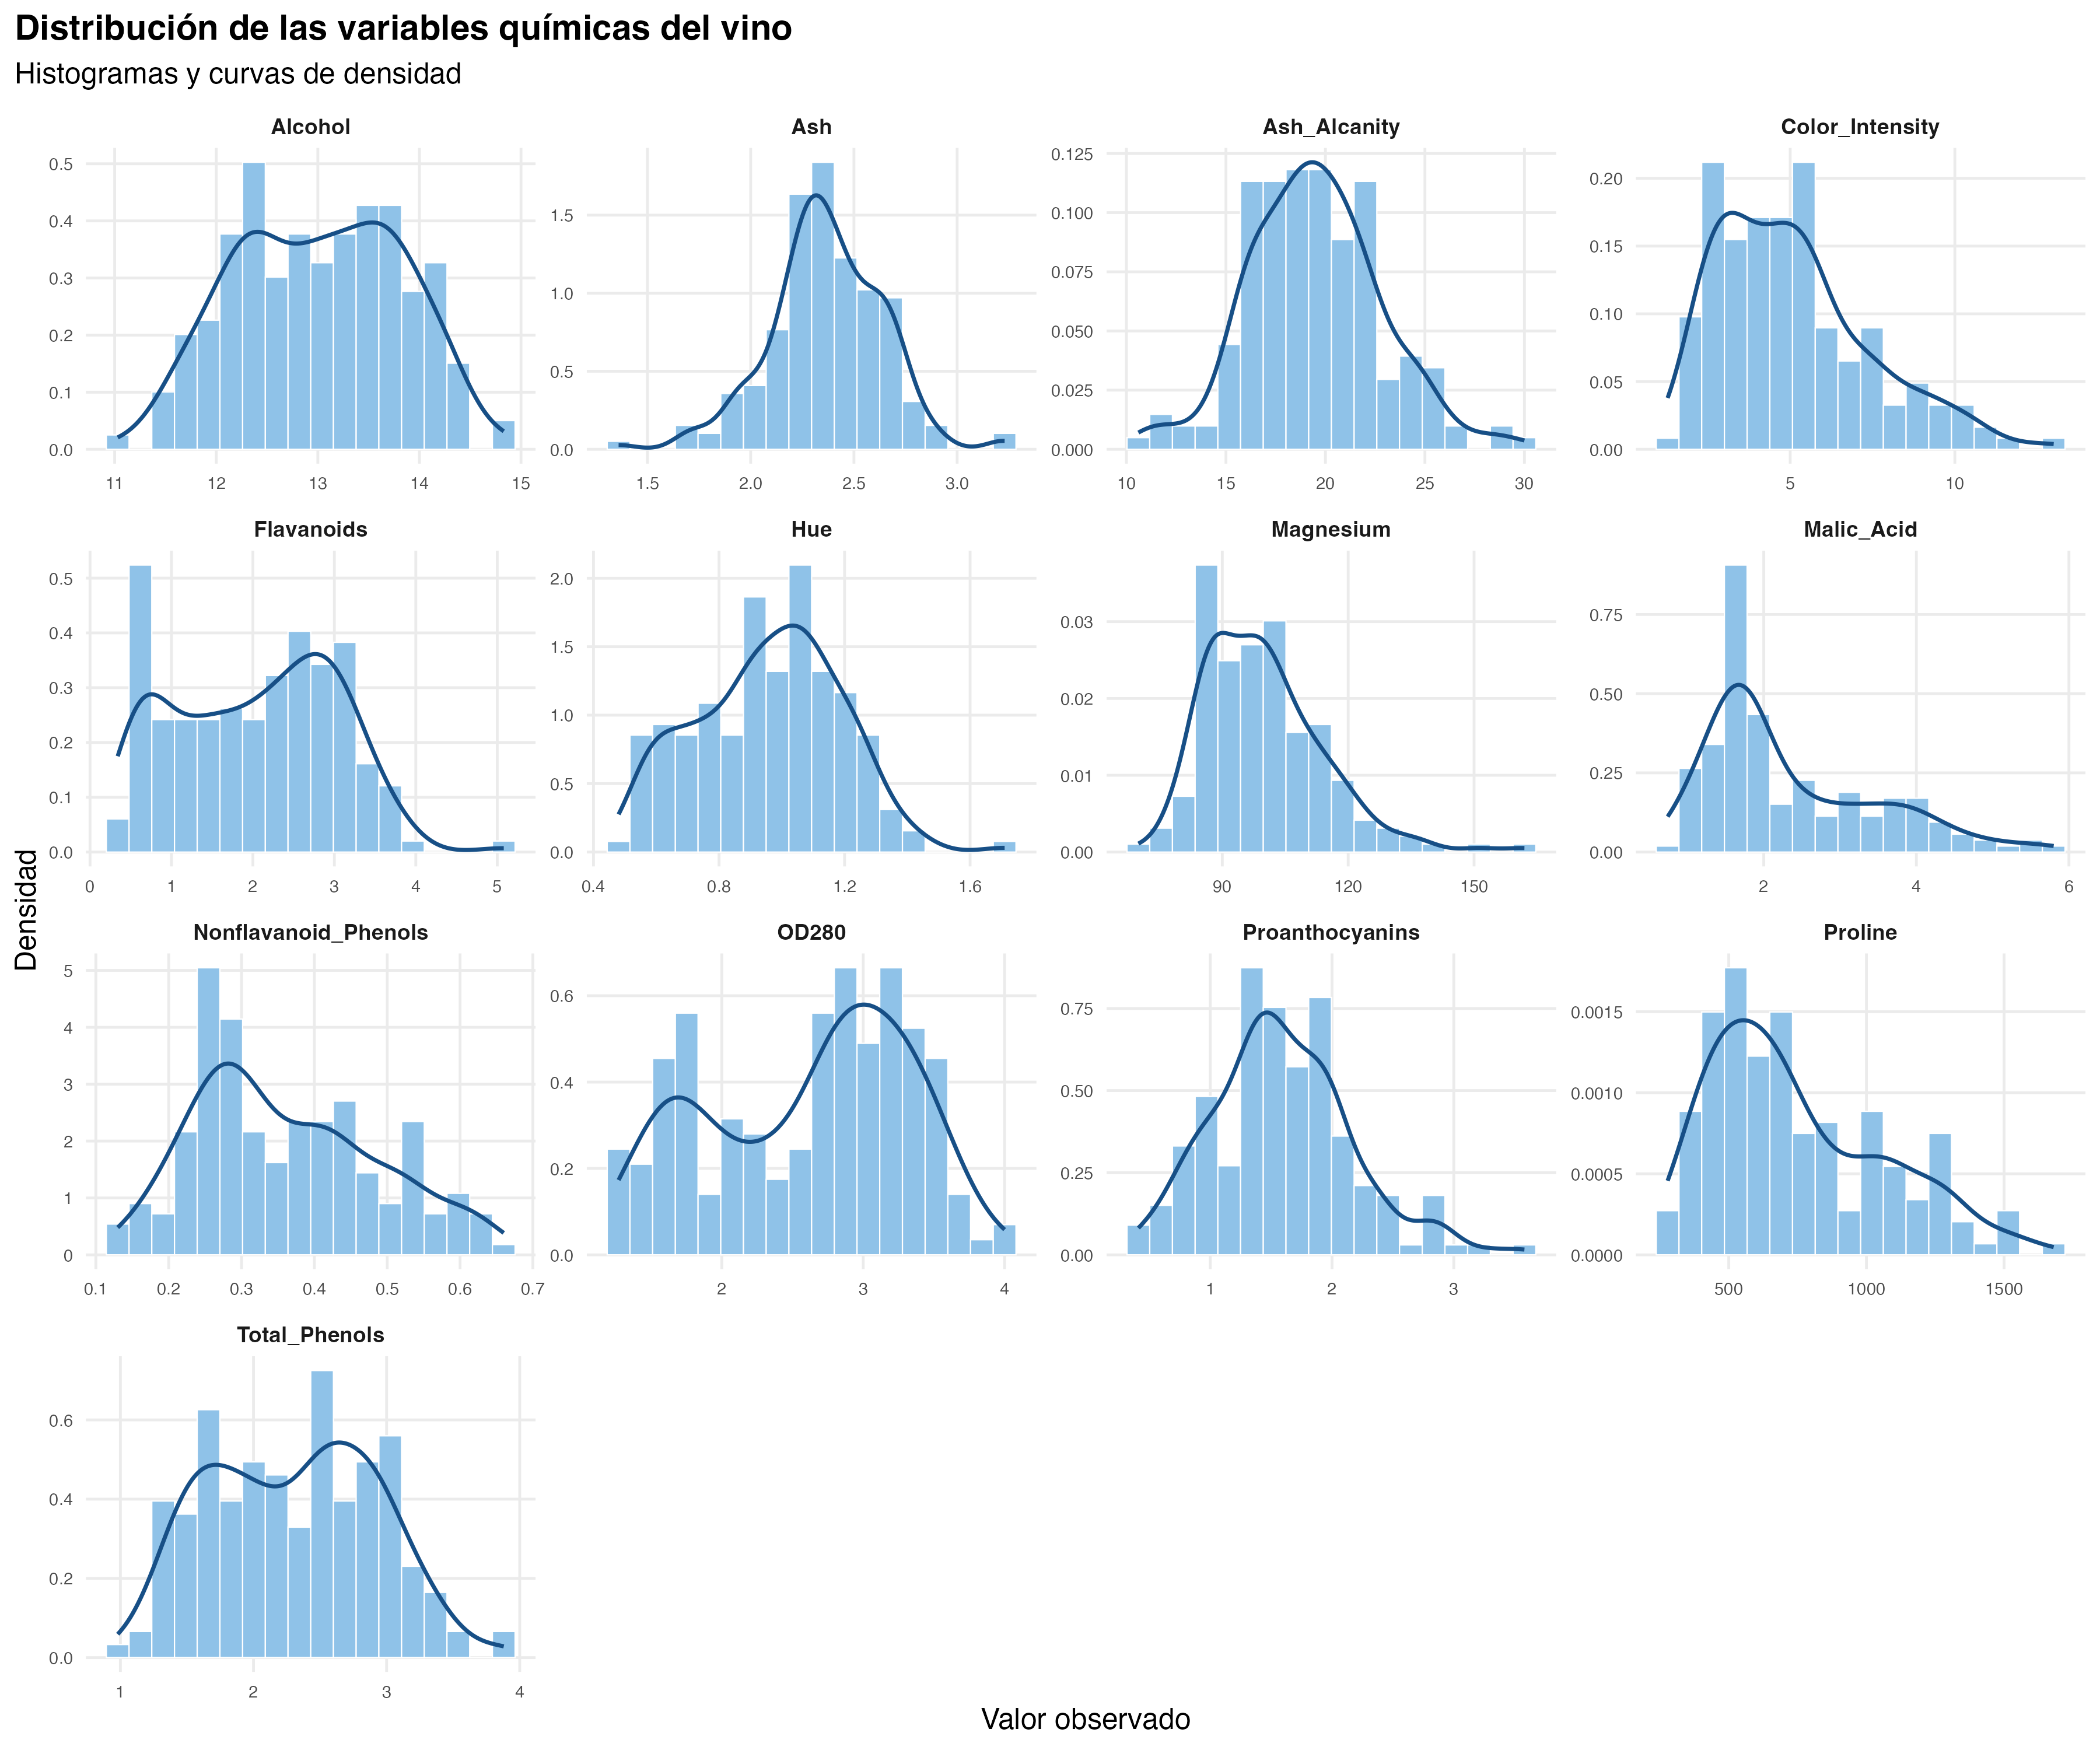
\includegraphics[width=0.86\textwidth]{09_distribuciones_variables.png}
  \caption{Histogramas (barras) y curvas de densidad (línea) de las 13 variables químicas. Cada panel tiene su propia escala en ambos ejes.}
  \label{fig:distribuciones}
\end{figure*}

\subsection{2.4 Comparación de dispersión y outliers}

\begin{lstlisting}[firstnumber=335]
# Como las variables tienen unidades diferentes, se estandarizan para poder
# compararlas en una misma gráfica de cajas.
datos_estandarizados <- wine %>%
  mutate(across(where(is.numeric), ~ as.numeric(scale(.x)))) %>%
  pivot_longer(
    cols = -Pueblo,
    names_to = "Variable",
    values_to = "Valor_estandarizado"
  )
\end{lstlisting}

\var{scale()} \textbf{estandariza} cada variable con \textit{z} = (\textit{x} − \textit{x̄}) / \textit{s}. Así todas quedan con media 0 y desviación estándar 1, y pueden compararse en una misma gráfica de cajas (Figura~\ref{fig:boxplots}).

\begin{figure}[htbp]
  \centering
  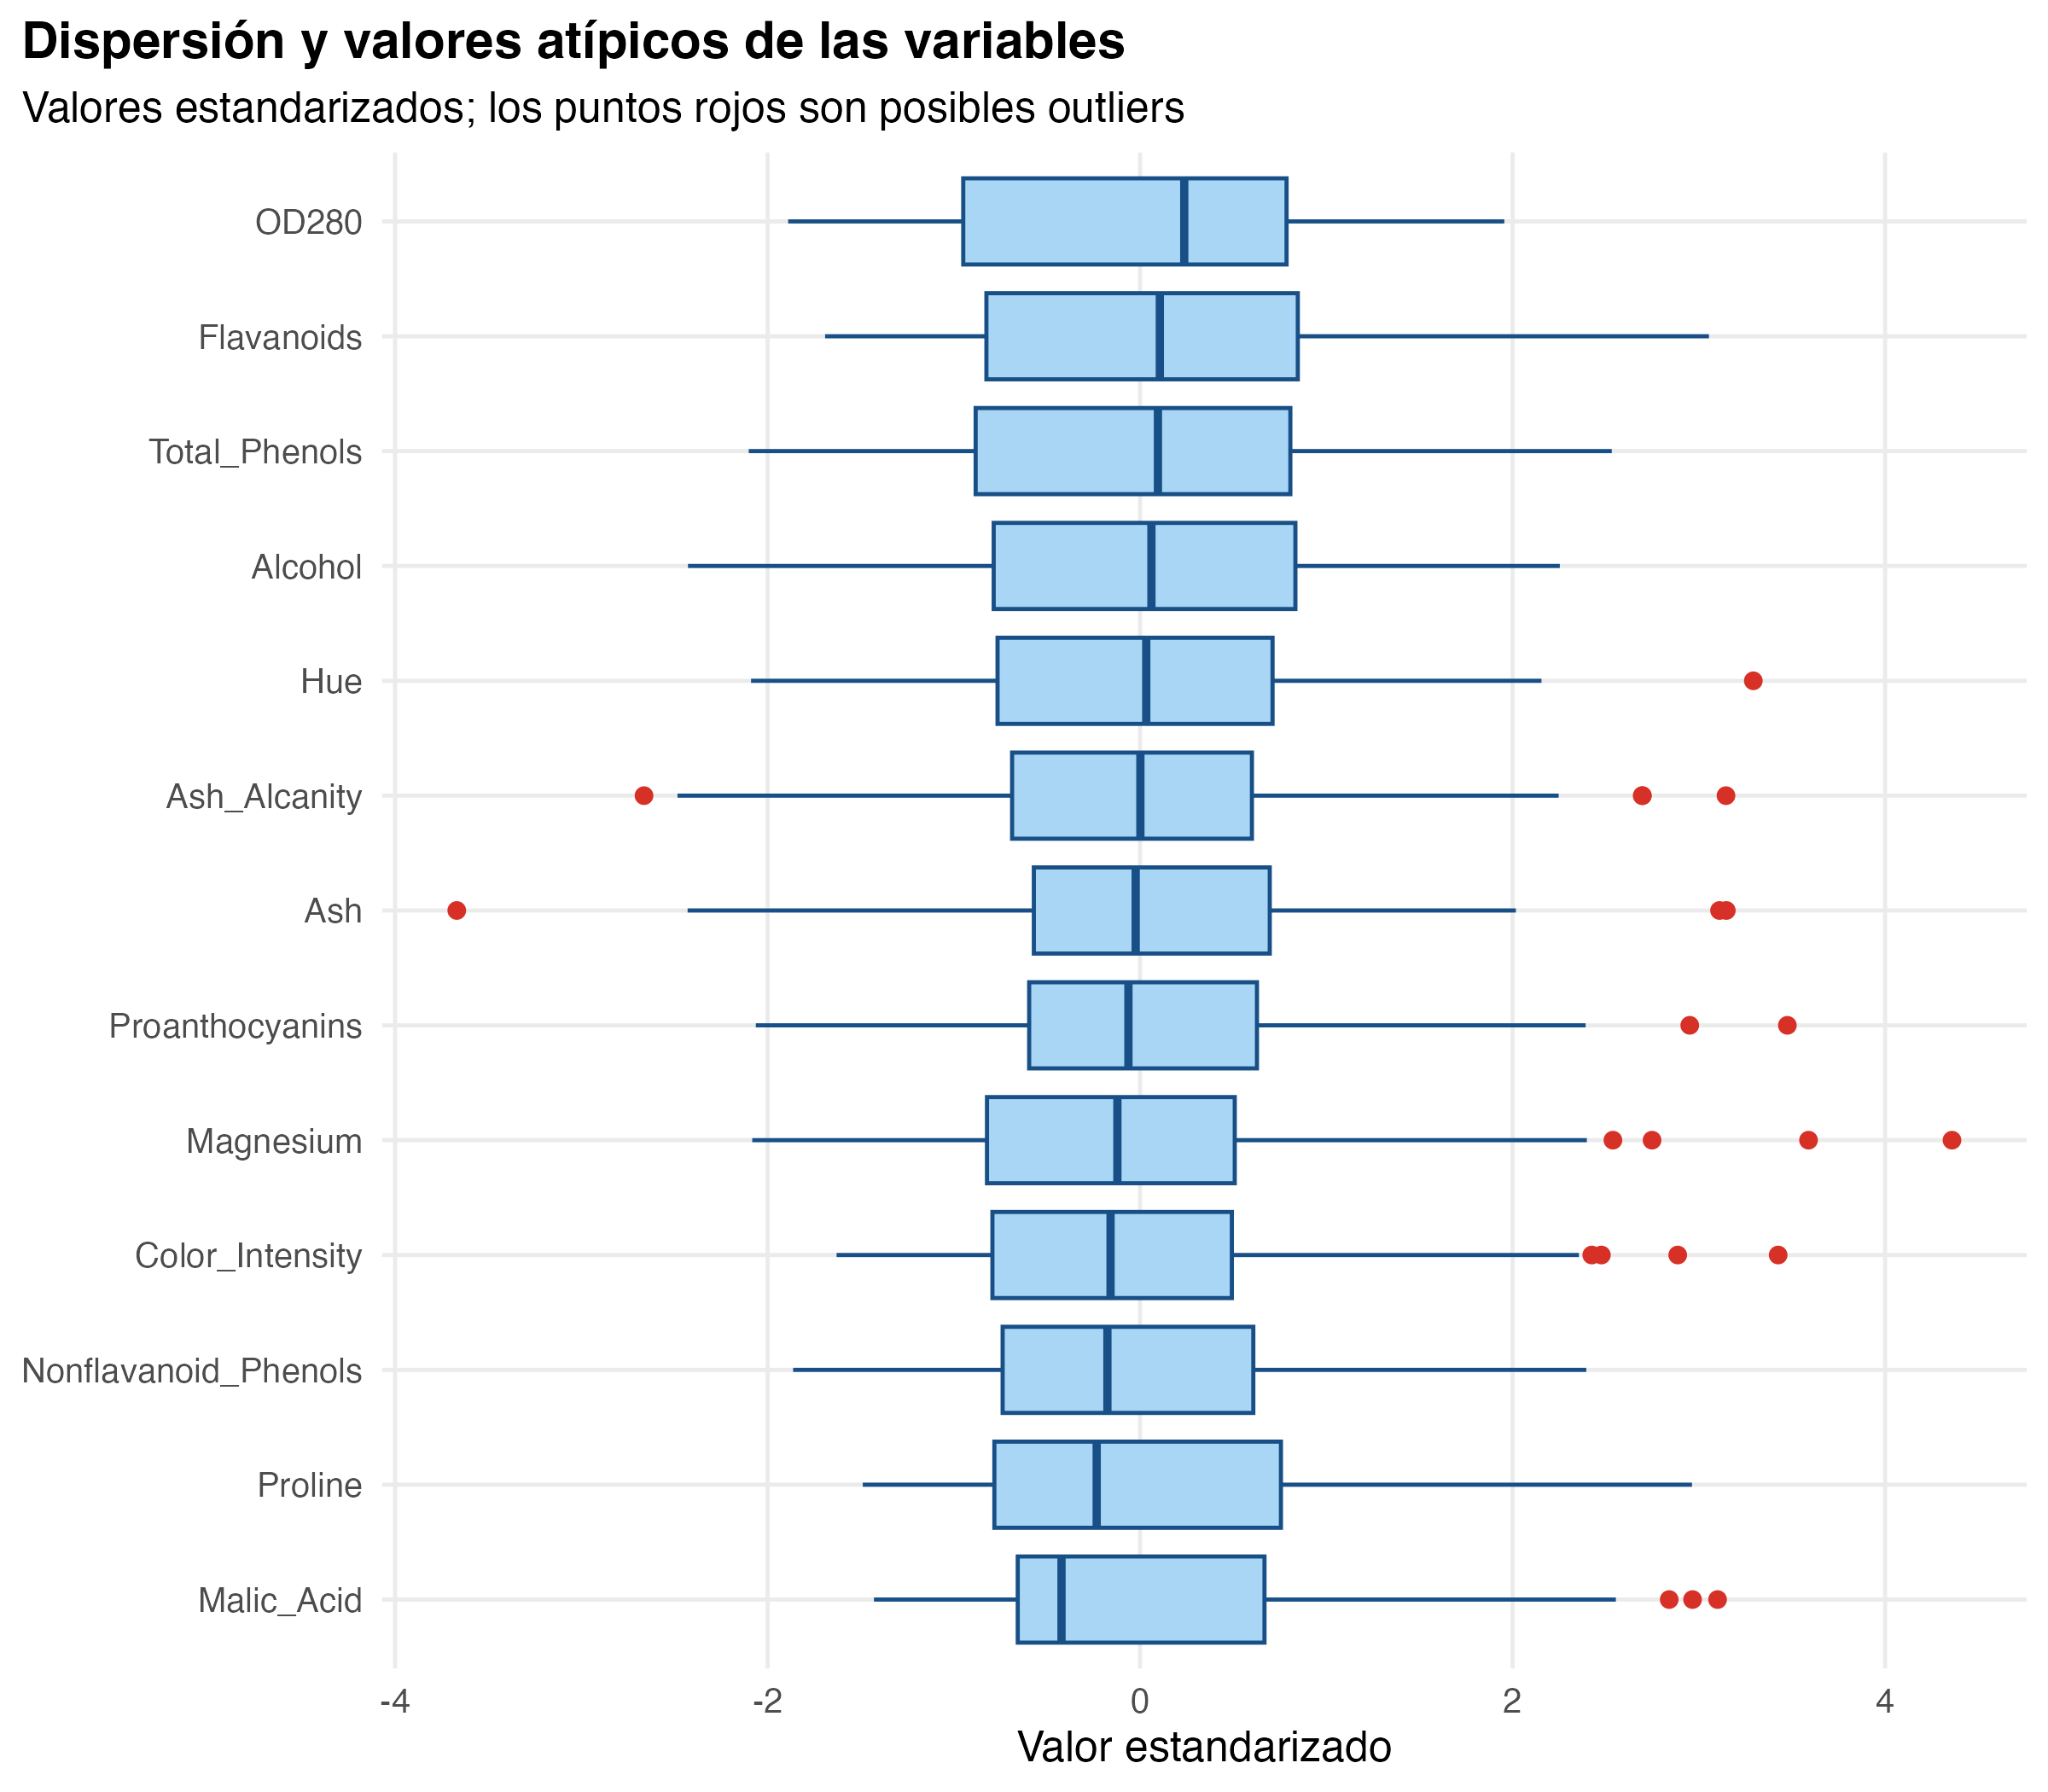
\includegraphics[width=\columnwidth]{10_boxplots_variables.png}
  \caption{Diagramas de caja de las variables estandarizadas. La caja abarca de Q1 a Q3, la línea interior es la mediana y los puntos son los valores atípicos según el criterio de Tukey.}
  \label{fig:boxplots}
\end{figure}

\subsection{2.5 Correlaciones entre variables}

\begin{lstlisting}[firstnumber=374]
# La correlación permite explorar asociaciones lineales y anticipar posibles
# problemas de multicolinealidad en la regresión del punto 3.
matriz_correlaciones <- wine %>%
  select(-Pueblo) %>%
  cor(use = "complete.obs")
\end{lstlisting}

El \textbf{coeficiente de correlación de Pearson} (\textit{r}) mide la asociación lineal entre dos variables y va de −1 a 1. Las correlaciones más altas fueron \var{Total\_Phenols}–\var{Flavanoids} (\textit{r} = 0.865), \var{Flavanoids}–\var{OD280} (0.787) y \var{Total\_Phenols}–\var{OD280} (0.700); las más negativas, \var{Malic\_Acid}–\var{Hue} (−0.561) y \var{Flavanoids}–\var{Nonflavanoid\_Phenols} (−0.538). Correlaciones altas entre predictores pueden causar \textit{multicolinealidad} en una regresión (Figura~\ref{fig:correlaciones}).

\begin{figure*}[tp]
  \centering
  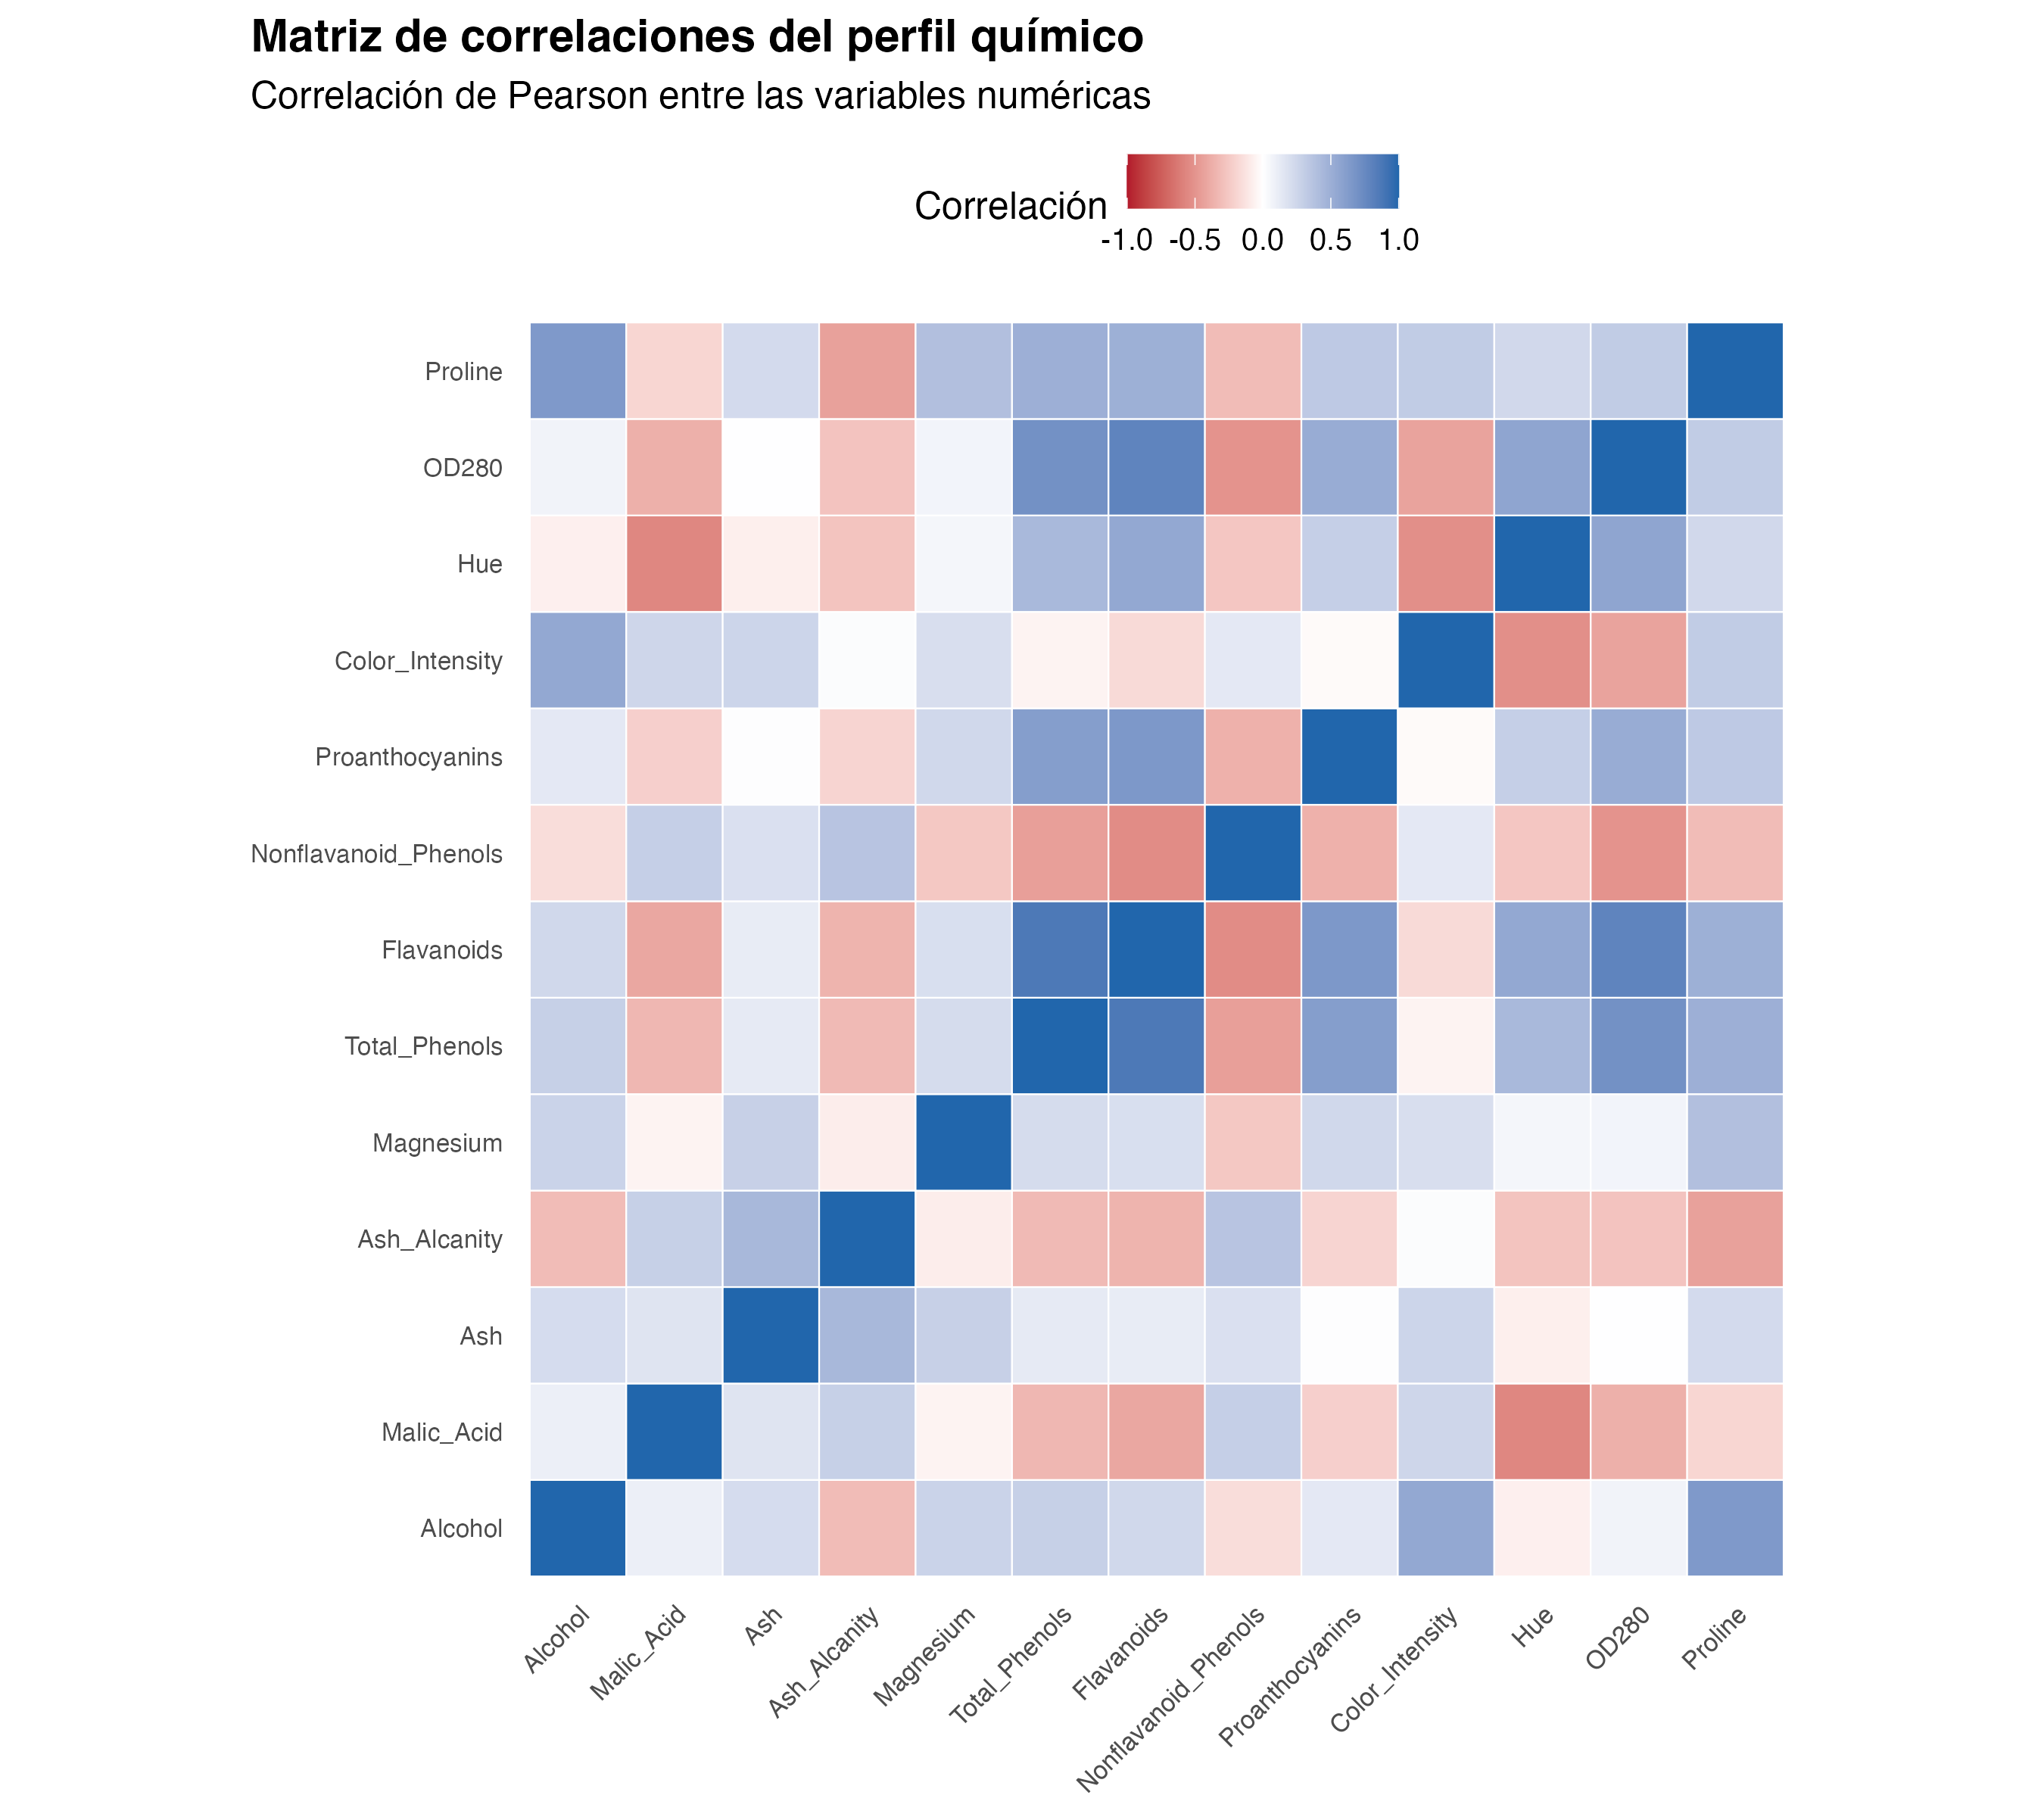
\includegraphics[width=0.62\textwidth]{11_matriz_correlaciones.png}
  \caption{Matriz de correlaciones de Pearson entre las 13 variables químicas. Cada celda muestra la correlación de un par de variables, de −1 a 1.}
  \label{fig:correlaciones}
\end{figure*}

\subsection{2.6 Variables principales para el punto 3}

\begin{lstlisting}[firstnumber=434]
variables_clave <- c(
  "Proline",
  "Alcohol",
  "Flavanoids",
  "Color_Intensity",
  "OD280",
  "Total_Phenols"
)
\end{lstlisting}

Se seleccionan seis variables para comparar visualmente los tres pueblos antes de aplicar las pruebas formales (Figura~\ref{fig:clave}).

\begin{figure*}[tp]
  \centering
  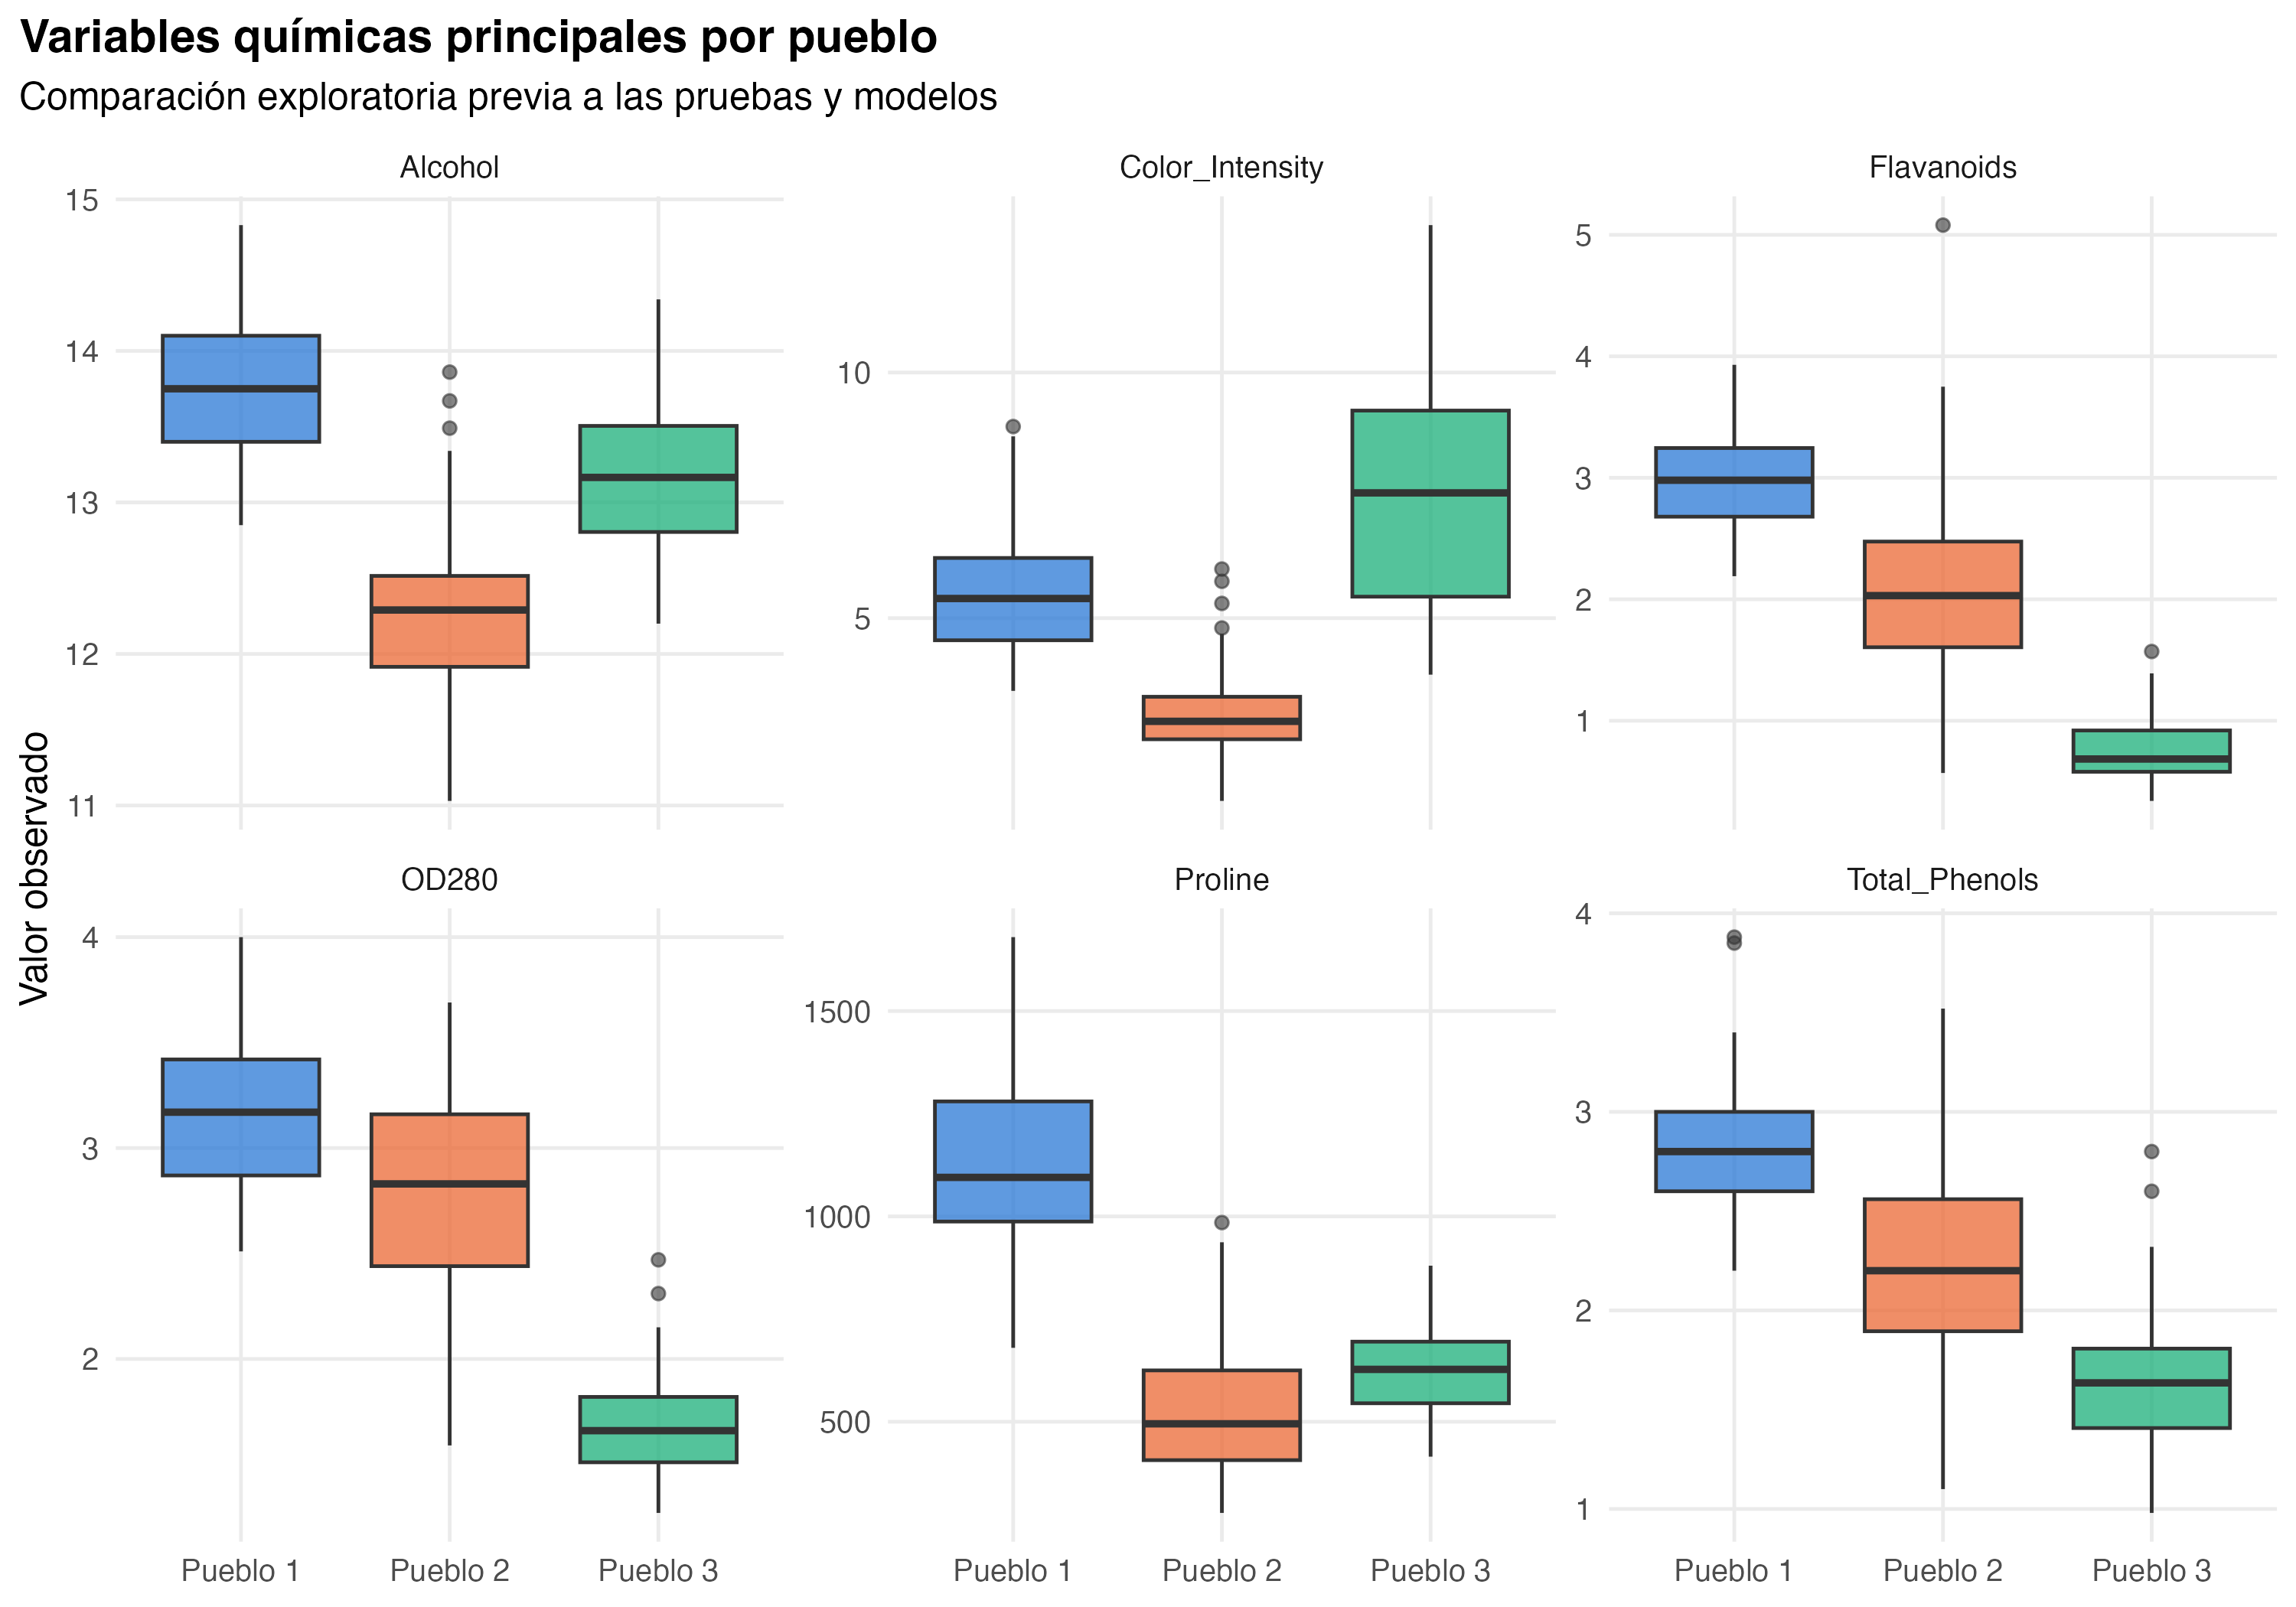
\includegraphics[width=0.80\textwidth]{12_variables_clave_por_pueblo.png}
  \caption{Diagramas de caja de seis variables principales en cada pueblo: \var{Alcohol}, \var{Color\_Intensity}, \var{Flavanoids}, \var{OD280}, \var{Proline} y \var{Total\_Phenols}.}
  \label{fig:clave}
\end{figure*}

% =======================================================================
\section{3. Inferencia estadística y modelos}

\begin{lstlisting}[firstnumber=479]
# Semilla para reproducir particiones, validación cruzada y modelos
set.seed(2026)
\end{lstlisting}

\var{set.seed()} fija el generador de números aleatorios, de modo que la partición de los datos y la validación cruzada producen siempre los mismos resultados.

\subsection{3.a Descripción de las pruebas y modelos}

\begin{enumerate}
  \item[3.1] \textbf{ANOVA de una vía} (y alternativas robustas) para comparar la prolina media entre pueblos.
  \item[3.2] \textbf{Kruskal-Wallis} por variable para identificar qué compuestos difieren entre pueblos.
  \item[3.3] \textbf{Regresión lineal múltiple} para predecir la prolina a partir de los demás compuestos.
  \item[3.4] \textbf{Regresión logística multinomial} para clasificar el pueblo de origen de una muestra.
\end{enumerate}

\subsection{3.1 Prolina por pueblo: ANOVA y supuestos}

\begin{lstlisting}[firstnumber=490]
# Media y desviación estándar de prolina por pueblo
wine %>% group_by(Pueblo) %>% get_summary_stats(Proline, type = "mean_sd")

# ANOVA clásico; H0: la prolina media es igual en los tres pueblos
anova_prolina <- aov(Proline ~ Pueblo, data = wine)
summary(anova_prolina)

# Supuestos: normalidad de residuos (Shapiro-Wilk) y homogeneidad de varianzas (Levene)
shapiro.test(residuals(anova_prolina))
leveneTest(Proline ~ Pueblo, data = wine)
\end{lstlisting}

El \textbf{ANOVA de una vía} compara las medias de tres o más grupos. Contrasta \Hcero: \textit{las medias de prolina son iguales en los tres pueblos}, mediante el estadístico \textit{F}, que compara la variación entre grupos con la variación dentro de cada grupo. Supone residuos normales y varianzas iguales entre grupos.

Las medias (± DE) fueron 1116 ± 222 mg/L (Pueblo~1), 520 ± 157 mg/L (Pueblo~2) y 630 ± 115 mg/L (Pueblo~3). Resultados:
\begin{itemize}
  \item ANOVA: \textit{F}(2, 175) = 207.9, \pval{} < \sci{2}{16}.
  \item Shapiro-Wilk sobre los residuos: \textit{W} = 0.982, \pval{} = 0.021, por lo que \textbf{no se cumple} la normalidad (Figura~\ref{fig:qq}).
  \item Levene: \textit{F}(2, 175) = 8.51, \pval{} = 0.0003, por lo que \textbf{no se cumple} la igualdad de varianzas.
\end{itemize}

\begin{figure}[htbp]
  \centering
  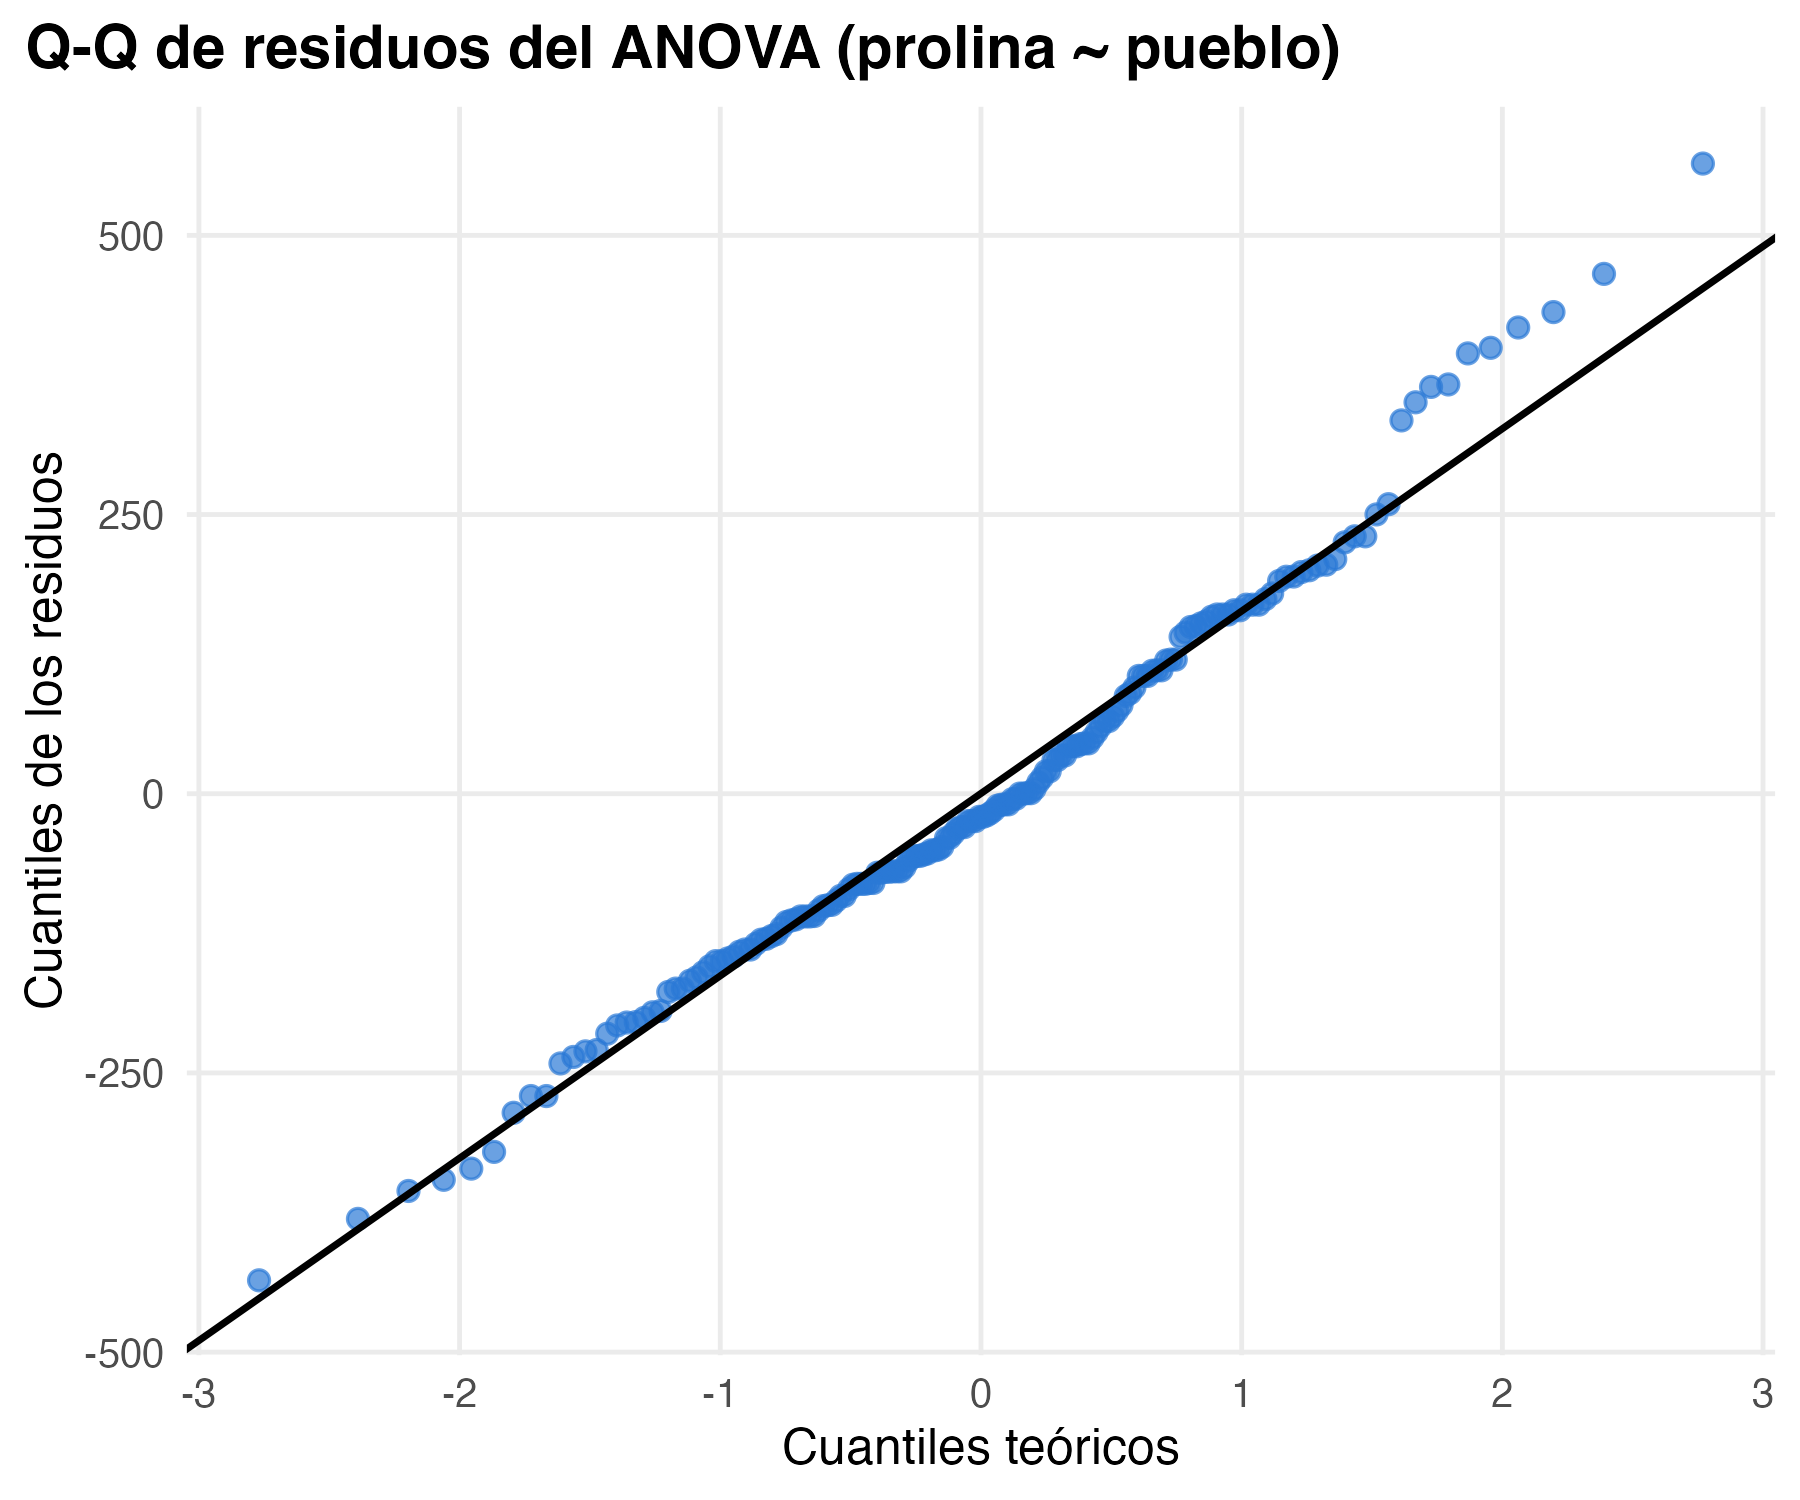
\includegraphics[width=0.85\columnwidth]{02_anova_qq_residuos.png}
  \caption{Gráfica Q-Q de los residuos del ANOVA. Si los residuos fueran normales, los puntos seguirían la línea recta.}
  \label{fig:qq}
\end{figure}

\begin{lstlisting}[firstnumber=511]
# Alternativas robustas ante violación de supuestos: ANOVA de Welch y Kruskal-Wallis (+ tamaño de efecto)
welch_anova_test(wine, Proline ~ Pueblo)
kruskal_test(wine, Proline ~ Pueblo)
kruskal_effsize(wine, Proline ~ Pueblo)

# Comparaciones por pares con Games-Howell (no asume varianzas iguales)
gh_prolina <- games_howell_test(wine, Proline ~ Pueblo) %>% mutate(p_lab = scales::pvalue(p.adj, add_p = TRUE))
gh_prolina
\end{lstlisting}

Como no se cumplen los supuestos, se aplican dos alternativas:
\begin{itemize}
  \item El \textbf{ANOVA de Welch}, que no asume varianzas iguales: \textit{F}(2, 111.8) = 153.8, \pval{} = \sci{7.9}{33}.
  \item La prueba de \textbf{Kruskal-Wallis}, que es no paramétrica y compara rangos en lugar de medias, por lo que no requiere normalidad: \textit{H}(2) = 119.1, \pval{} = \sci{1.4}{26}.
\end{itemize}
El \textbf{tamaño del efecto} \etaH{} = (\textit{H} − \textit{k} + 1) / (\textit{n} − \textit{k}) indica la proporción de la variabilidad explicada por el pueblo: \etaH{} = 0.669, clasificado como \textit{grande} (≥ 0.14).

La prueba de \textbf{Games-Howell} compara los pueblos por pares sin asumir varianzas iguales (Figura~\ref{fig:prolina}):
\begin{itemize}
  \item Pueblo 2 − Pueblo 1: −596.2 mg/L [IC 95\,\%: −677.9, −514.5], \pval{} < 0.001.
  \item Pueblo 3 − Pueblo 1: −485.8 mg/L [−565.1, −406.5], \pval{} < 0.001.
  \item Pueblo 3 − Pueblo 2: 110.4 mg/L [51.1, 169.7], \pval{} < 0.001.
\end{itemize}

\begin{figure}[htbp]
  \centering
  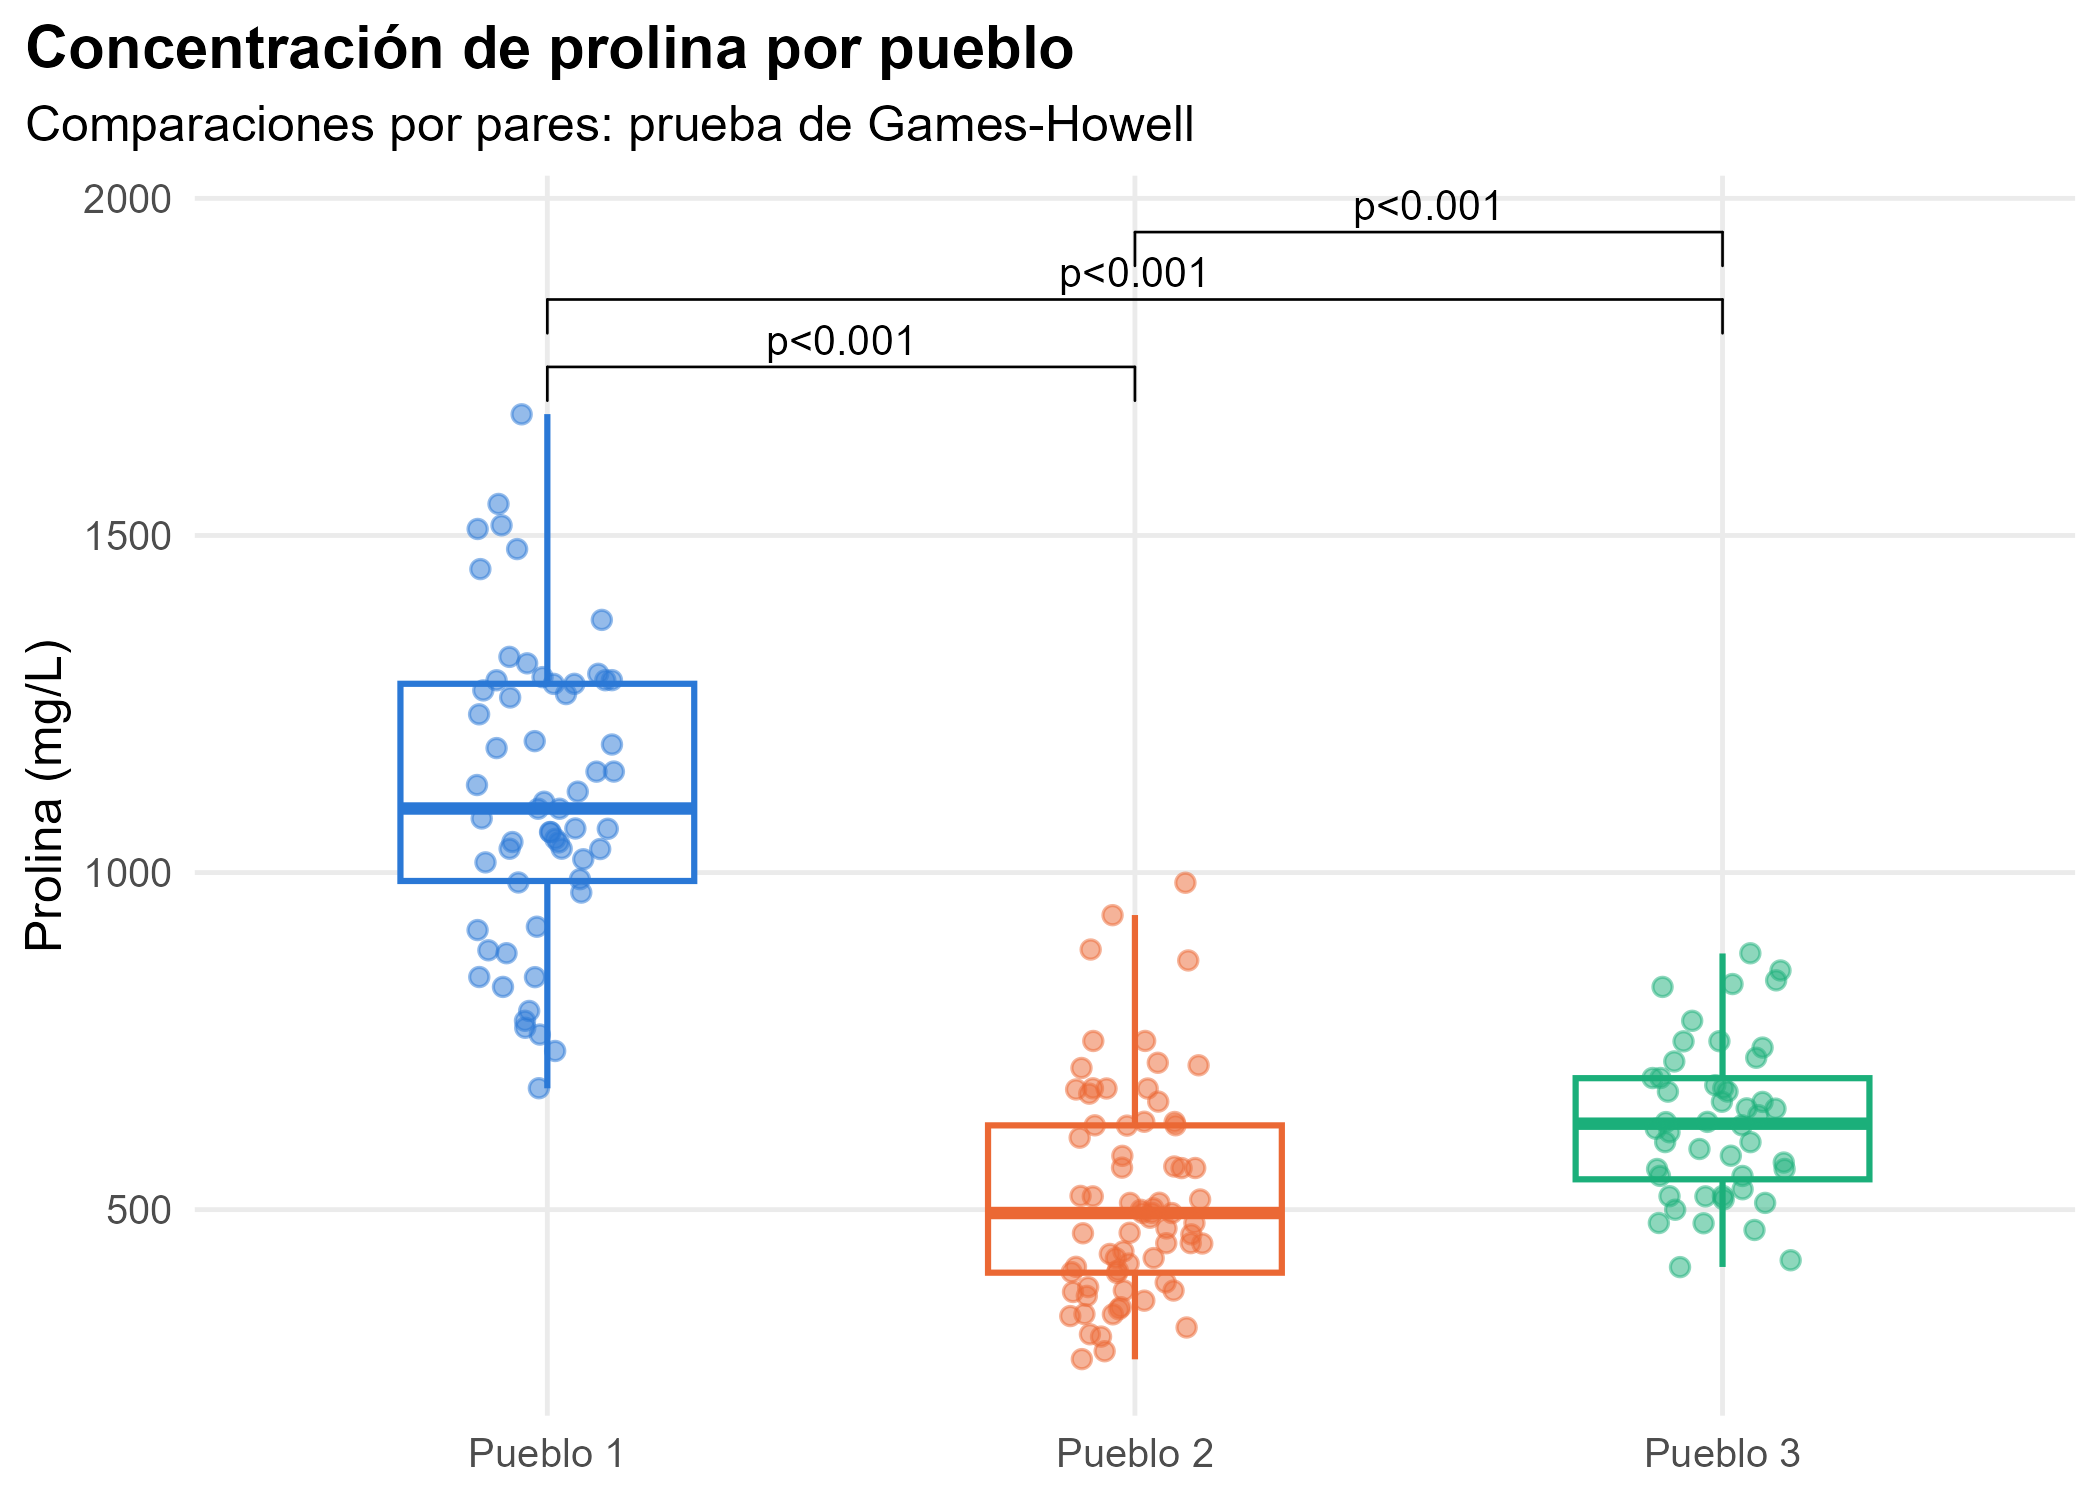
\includegraphics[width=\columnwidth]{03_prolina_por_pueblo.png}
  \caption{Concentración de prolina (mg/L) en cada pueblo. Los puntos son las muestras individuales y los corchetes superiores muestran los \textit{p}-valores ajustados de Games-Howell para cada par de pueblos.}
  \label{fig:prolina}
\end{figure}

\subsection{3.2 Kruskal-Wallis por variable}

\begin{lstlisting}[firstnumber=534]
# Kruskal-Wallis y eta² (η²[H]) para cada variable química, con p-valores ajustados por Bonferroni
kw_variables <- wine %>%
  pivot_longer(-Pueblo, names_to = "Variable", values_to = "Valor") %>%
  group_by(Variable) %>%
  summarise(H = kruskal.test(Valor ~ Pueblo)$statistic,
            p = kruskal.test(Valor ~ Pueblo)$p.value,
            eta2_H = kruskal_effsize(pick(everything()), Valor ~ Pueblo)$effsize) %>%
  mutate(p_ajustado = p.adjust(p, method = "bonferroni")) %>%
  arrange(desc(eta2_H))
kw_variables
\end{lstlisting}

Se aplica Kruskal-Wallis a cada una de las 13 variables. Hacer muchas pruebas a la vez aumenta la probabilidad de obtener algún falso positivo. La corrección de \textbf{Bonferroni} lo compensa multiplicando cada \pval{} por el número de pruebas (13). Las 13 variables obtuvieron \pval{} ajustado < 0.001. Solo \var{Ash} quedó por debajo del umbral de efecto grande, con \etaH{} = 0.121 (Tabla~\ref{tab:kw}, Figura~\ref{fig:kw}).

\begin{table}[htbp]
  \centering
  \caption{Kruskal-Wallis por variable (gl = 2), ordenado por tamaño de efecto.}
  \label{tab:kw}
  \footnotesize
  \begin{tabular}{@{}lrrr@{}}
    \toprule
    \textbf{Variable} & \textbf{\textit{H}} & \textbf{\etaH} & \textbf{\textit{p} ajustado} \\
    \midrule
    \var{Flavanoids}           & 130.45 & 0.734 & \sci{6.12}{28} \\
    \var{Proline}              & 119.06 & 0.669 & \sci{1.82}{25} \\
    \var{Color\_Intensity}     & 115.05 & 0.646 & \sci{1.35}{24} \\
    \var{Alcohol}              & 109.51 & 0.614 & \sci{2.16}{23} \\
    \var{OD280}                & 107.05 & 0.600 & \sci{7.40}{23} \\
    \var{Total\_Phenols}       & 93.48  & 0.523 & \sci{6.54}{20} \\
    \var{Hue}                  & 92.44  & 0.517 & \sci{1.10}{19} \\
    \var{Ash\_Alcanity}        & 59.99  & 0.331 & \sci{1.22}{12} \\
    \var{Proanthocyanins}      & 59.47  & 0.328 & \sci{1.58}{12} \\
    \var{Malic\_Acid}          & 50.04  & 0.275 & \sci{1.77}{10} \\
    \var{Magnesium}            & 40.58  & 0.220 & \sci{2.01}{8} \\
    \var{Nonflav.\_Phenols}    & 39.86  & 0.216 & \sci{2.88}{8} \\
    \var{Ash}                  & 23.13  & 0.121 & \sci{1.23}{4} \\
    \bottomrule
  \end{tabular}
\end{table}

\begin{figure}[htbp]
  \centering
  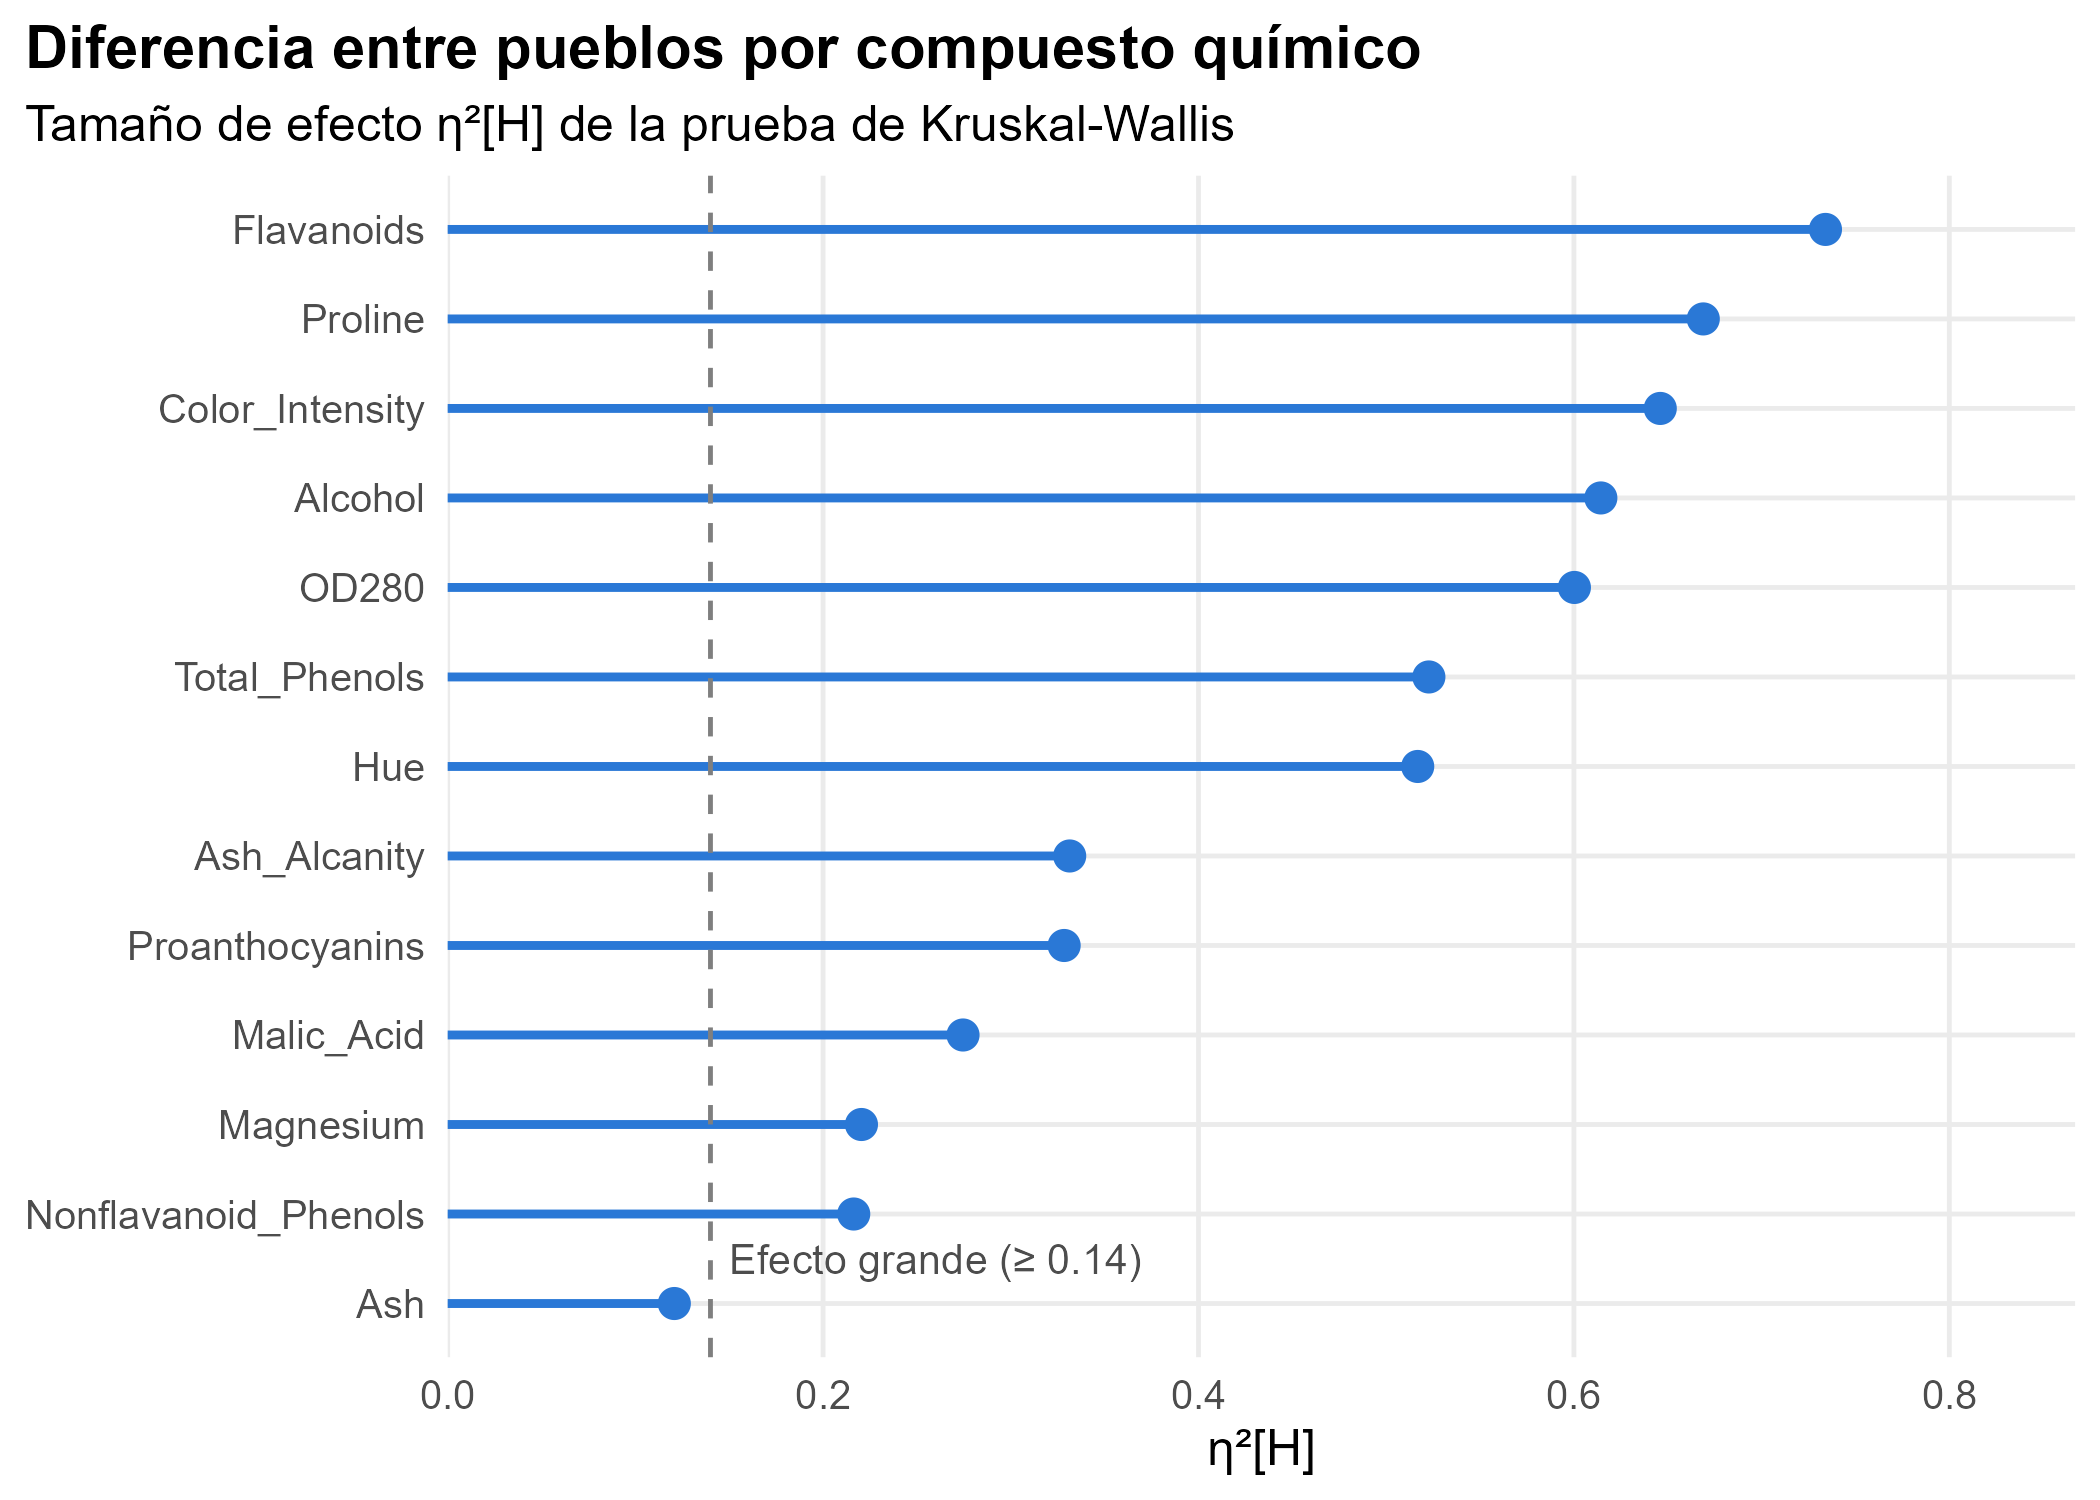
\includegraphics[width=\columnwidth]{04_kruskal_efecto_por_variable.png}
  \caption{Tamaño de efecto \etaH{} de la prueba de Kruskal-Wallis para cada variable. La línea discontinua marca el umbral de efecto grande (0.14).}
  \label{fig:kw}
\end{figure}

\subsection{3.3 Regresión lineal múltiple: prolina}

\begin{lstlisting}[firstnumber=560]
# Partición estratificada 70/30 por pueblo (la misma se reutiliza en 3.4)
idx_train <- createDataPartition(wine$Pueblo, p = 0.7, list = FALSE)
train <- wine[idx_train, ]
test  <- wine[-idx_train, ]

# Modelo completo con los 12 compuestos (sin el pueblo) y selección de variables por AIC en ambos sentidos
lm_completo <- lm(Proline ~ . - Pueblo, data = train)
lm_prolina  <- MASS::stepAIC(lm_completo, direction = "both", trace = FALSE)
summary(lm_prolina)
\end{lstlisting}

Los datos se dividen en \textbf{entrenamiento} (70\,\%, 126 muestras) y \textbf{prueba} (30\,\%, 52 muestras), manteniendo la proporción de cada pueblo. Una \textbf{regresión lineal múltiple} modela la prolina como una suma ponderada de los otros 12 compuestos. \var{stepAIC()} agrega y quita variables mientras el \textbf{criterio de información de Akaike} (AIC) disminuya; el AIC equilibra el ajuste del modelo contra su número de parámetros. El modelo final conservó 8 variables (Tabla~\ref{tab:regresion}): \textit{R}² = 0.636, \textit{R}² ajustado = 0.611, \textit{F}(8, 117) = 25.52, \pval{} < \sci{2.2}{16} y error estándar residual = 190.2 mg/L.

\begin{table}[htbp]
  \centering
  \caption{Coeficientes del modelo final para \var{Proline}.}
  \label{tab:regresion}
  \footnotesize
  \begin{tabular}{@{}lrrrr@{}}
    \toprule
    \textbf{Término} & \textbf{Estimado} & \textbf{EE} & \textbf{\textit{t}} & \textbf{\textit{p}} \\
    \midrule
    (Intercepto)            & −1190.78 & 410.38 & −2.90 & 0.0044 \\
    \var{Alcohol}           & 81.54    & 31.32  & 2.60  & 0.0104 \\
    \var{Ash}               & 248.78   & 90.09  & 2.76  & 0.0067 \\
    \var{Ash\_Alcanity}     & −23.57   & 7.26   & −3.24 & 0.0015 \\
    \var{Magnesium}         & 2.58     & 1.34   & 1.92  & 0.0570 \\
    \var{Flavanoids}        & 69.05    & 26.92  & 2.57  & 0.0116 \\
    \var{Nonflav.\_Phenols} & −275.10  & 185.55 & −1.48 & 0.1409 \\
    \var{Color\_Intensity}  & 38.50    & 11.36  & 3.39  & 0.0010 \\
    \var{Hue}               & 270.86   & 104.85 & 2.58  & 0.0110 \\
    \bottomrule
  \end{tabular}
\end{table}

Cada coeficiente indica cuánto cambia la prolina predicha (mg/L) al aumentar en una unidad esa variable, manteniendo las demás constantes.

\begin{lstlisting}[firstnumber=570]
# Supuestos: multicolinealidad (VIF > 5 preocupante), heterocedasticidad (Breusch-Pagan) y normalidad de residuos
vif(lm_prolina)
ncvTest(lm_prolina)
shapiro.test(residuals(lm_prolina))
\end{lstlisting}

Se verifican tres supuestos del modelo (Figura~\ref{fig:diagnostico}):
\begin{itemize}
  \item \textbf{Multicolinealidad}: el factor de inflación de la varianza (VIF) indica cuánto se infla la varianza de un coeficiente por su correlación con los demás predictores. El VIF máximo fue 2.65 (\var{Color\_Intensity}), menor que 5.
  \item \textbf{Homocedasticidad} (varianza constante de los residuos): Breusch-Pagan, χ²(1) = 2.95, \pval{} = 0.086, por lo que no se rechaza \Hcero.
  \item \textbf{Normalidad de residuos}: Shapiro-Wilk, \textit{W} = 0.992, \pval{} = 0.676, por lo que no se rechaza \Hcero.
\end{itemize}

\begin{figure*}[tp]
  \centering
  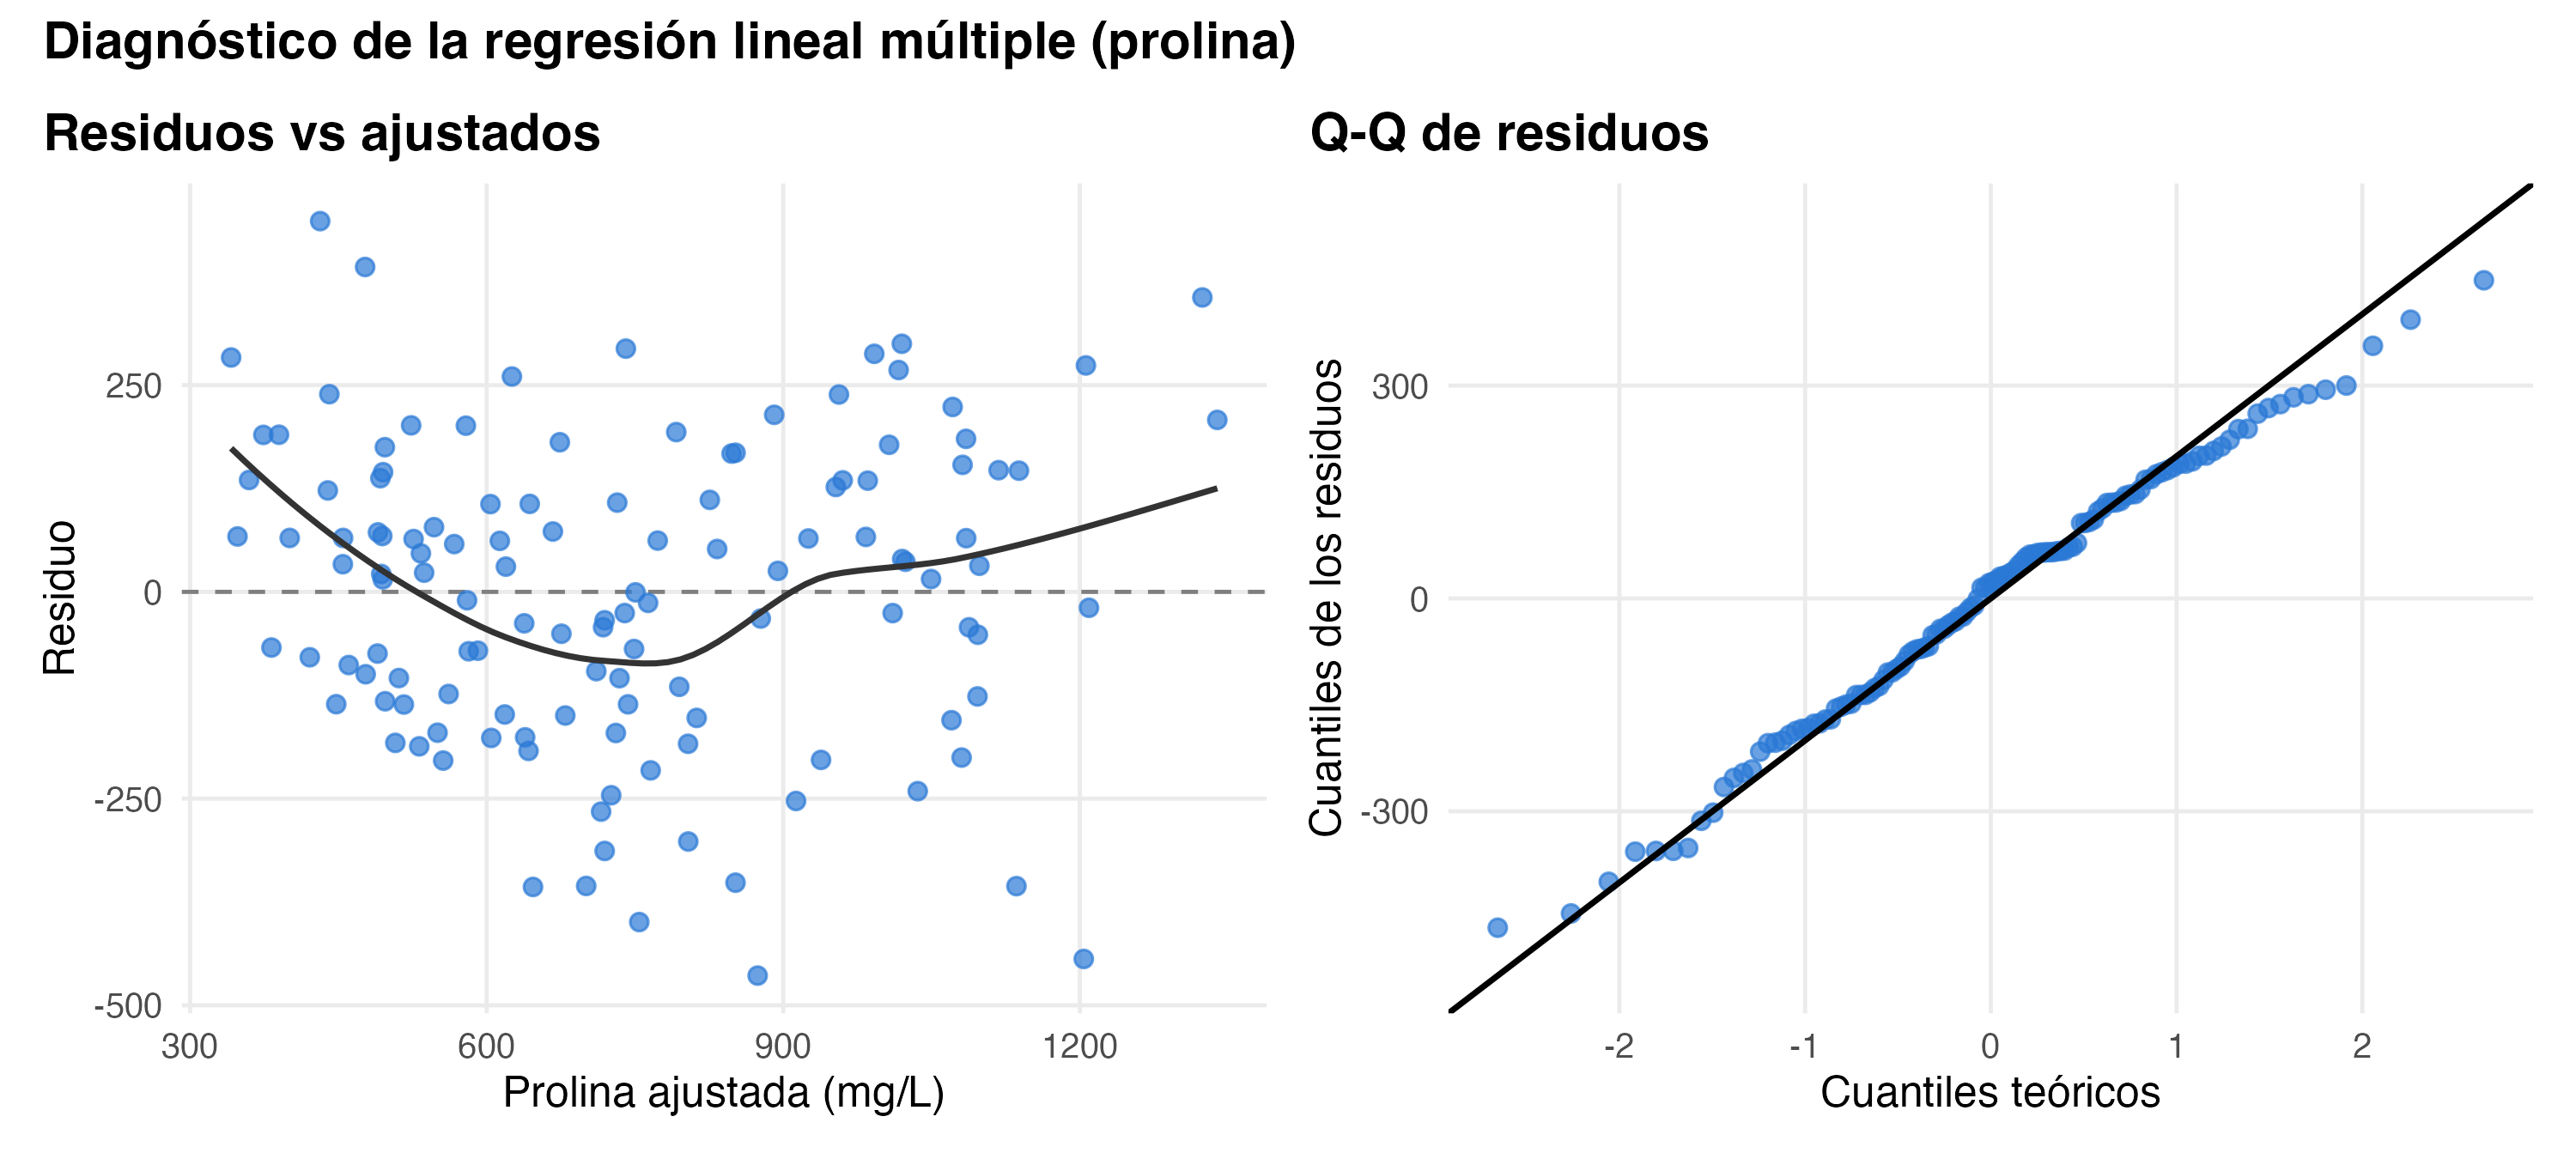
\includegraphics[width=0.90\textwidth]{05_regresion_diagnostico.png}
  \caption{Diagnóstico de la regresión lineal múltiple. Izquierda: residuos contra valores ajustados, con una curva de suavizado; se espera una nube sin patrón alrededor de 0. Derecha: gráfica Q-Q de los residuos.}
  \label{fig:diagnostico}
\end{figure*}

\begin{lstlisting}[firstnumber=593]
# Desempeño en el conjunto de prueba: RMSE, R² y MAE
pred_prolina <- predict(lm_prolina, newdata = test)
postResample(pred = pred_prolina, obs = test$Proline)
\end{lstlisting}

El modelo se evalúa con las 52 muestras de prueba, que no se usaron para ajustarlo:
\begin{itemize}
  \item \textbf{RMSE} (raíz del error cuadrático medio) = 210.8 mg/L.
  \item \textbf{MAE} (error absoluto medio) = 162.2 mg/L.
  \item \textit{R}² = 0.613.
\end{itemize}
El RMSE penaliza más los errores grandes que el MAE (Figura~\ref{fig:predicho}).

\begin{figure}[htbp]
  \centering
  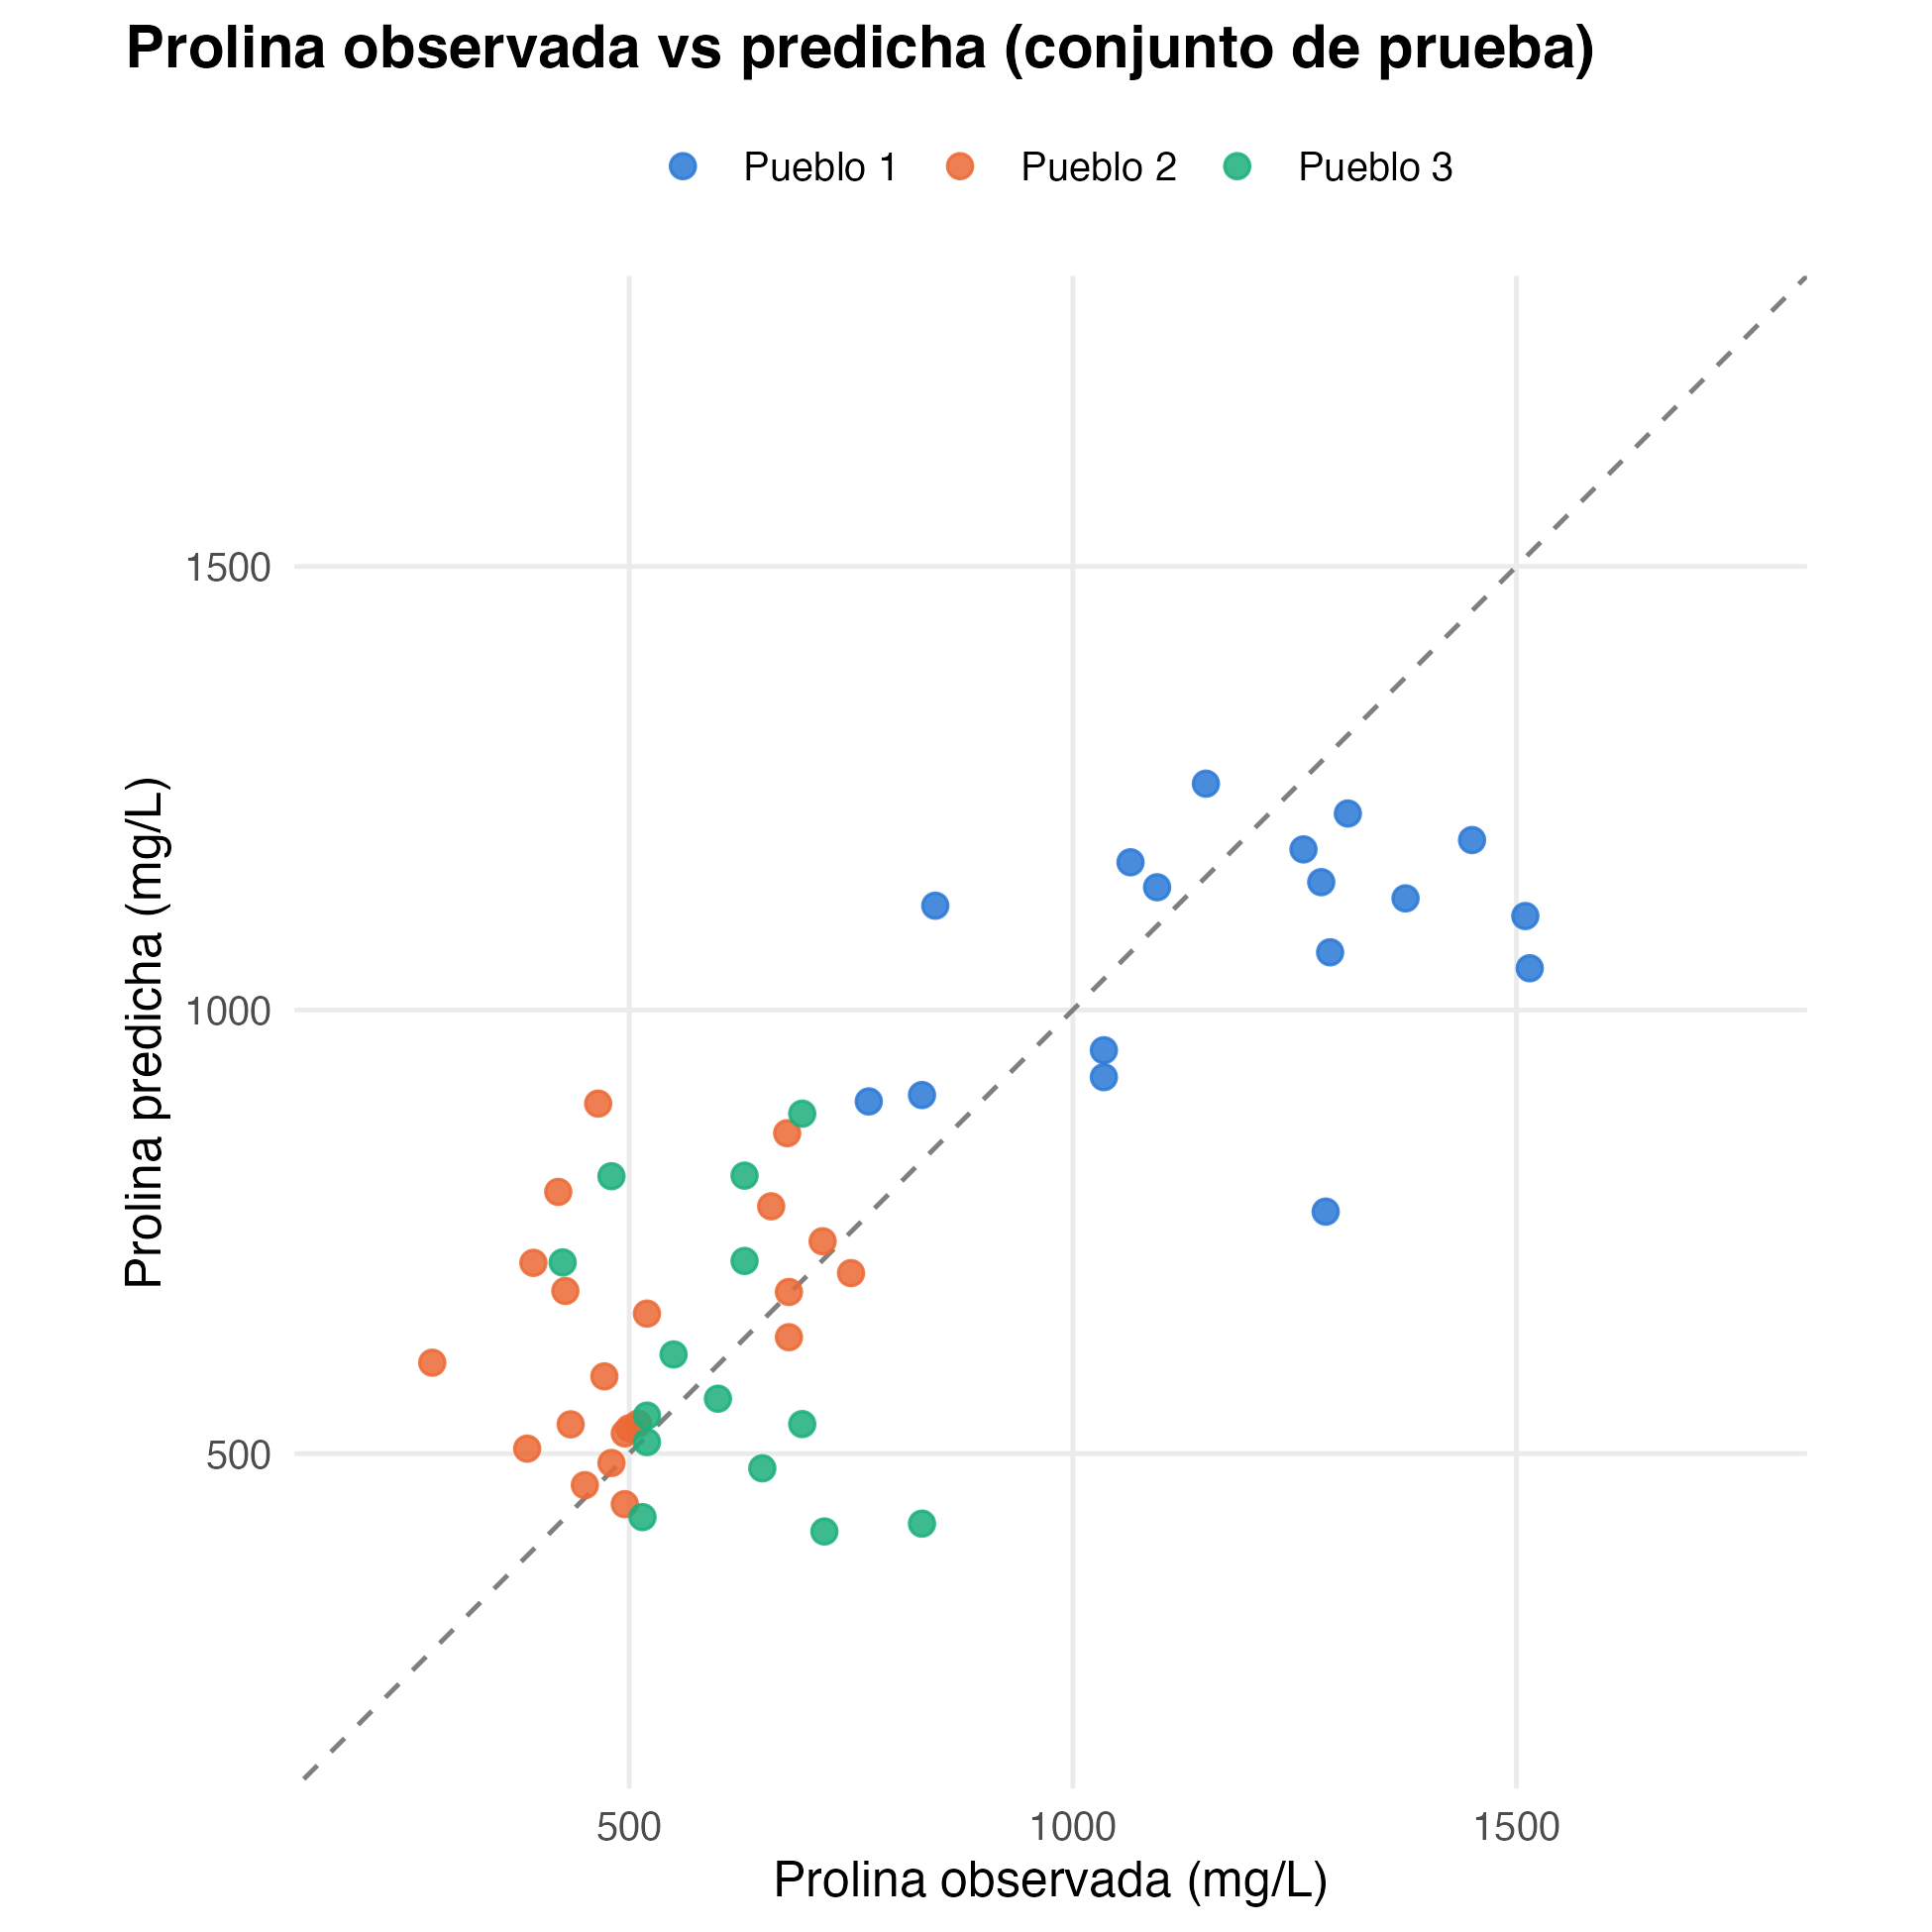
\includegraphics[width=0.88\columnwidth]{06_regresion_observado_vs_predicho.png}
  \caption{Prolina observada contra prolina predicha en el conjunto de prueba (52 muestras), por pueblo. La diagonal discontinua representa una predicción perfecta.}
  \label{fig:predicho}
\end{figure}

\subsection{3.4 Regresión logística multinomial: pueblo}

\begin{lstlisting}[firstnumber=612]
# Validación cruzada 10-fold sobre entrenamiento; estandariza predictores y ajusta la penalización (decay)
ctrl <- trainControl(method = "cv", number = 10)
multi_pueblo <- train(Pueblo ~ ., data = train, method = "multinom",
                      preProcess = c("center", "scale"), trControl = ctrl,
                      tuneGrid = expand.grid(decay = c(0, 0.001, 0.01, 0.1, 0.5, 1)), trace = FALSE)
multi_pueblo
\end{lstlisting}

La \textbf{regresión logística multinomial} estima la probabilidad de que una muestra pertenezca a cada uno de los tres pueblos a partir de las 13 variables químicas. Los predictores se estandarizan. El parámetro \var{decay} es una \textbf{penalización} que reduce el tamaño de los coeficientes para evitar el sobreajuste, y su valor se eligió con \textbf{validación cruzada de 10 pliegues}: el entrenamiento se divide en 10 partes y cada una se usa una vez como validación. El valor elegido fue \var{decay} = 0.001, con exactitud promedio de 1.000 en la validación cruzada.

\begin{lstlisting}[firstnumber=619]
# Razones de momios por cada desviación estándar de aumento (referencia: Pueblo 1)
exp(coef(multi_pueblo$finalModel))
\end{lstlisting}

Al exponenciar los coeficientes se obtienen \textbf{razones de momios} respecto al Pueblo~1. Un valor mayor que 1 indica que, al aumentar la variable en una desviación estándar, aumentan los momios de pertenecer a ese pueblo frente al Pueblo~1. Por ejemplo: 75.04 para \var{Ash\_Alcanity} (Pueblo~2) y 17.55 para \var{Color\_Intensity} (Pueblo~3).

\begin{lstlisting}[firstnumber=622]
# Desempeño en prueba: matriz de confusión, exactitud, kappa y métricas por clase
pred_pueblo <- predict(multi_pueblo, newdata = test)
cm_pueblo <- confusionMatrix(pred_pueblo, test$Pueblo)
cm_pueblo
\end{lstlisting}

La \textbf{matriz de confusión} cruza el pueblo real con el predicho (Figura~\ref{fig:confusion}). En prueba se clasificaron correctamente 51 de 52 muestras:
\begin{itemize}
  \item \textbf{Exactitud} = 0.981 [IC 95\,\%: 0.897, 0.9995], contra una tasa sin información (NIR) de 0.404 (\pval{} < \sci{2.2}{16}).
  \item \textbf{Kappa de Cohen} = 0.971. El kappa mide el acuerdo entre lo real y lo predicho, descontando el acuerdo esperado por azar.
\end{itemize}
La Tabla~\ref{tab:clases} resume las métricas por clase.

\begin{table}[htbp]
  \centering
  \caption{Métricas por clase en el conjunto de prueba.}
  \label{tab:clases}
  \footnotesize
  \begin{tabular}{@{}lccc@{}}
    \toprule
    \textbf{Métrica} & \textbf{Pueblo 1} & \textbf{Pueblo 2} & \textbf{Pueblo 3} \\
    \midrule
    Sensibilidad         & 1.000 & 0.952 & 1.000 \\
    Especificidad        & 1.000 & 1.000 & 0.974 \\
    Exactitud balanceada & 1.000 & 0.976 & 0.987 \\
    \bottomrule
  \end{tabular}
\end{table}

\begin{figure}[htbp]
  \centering
  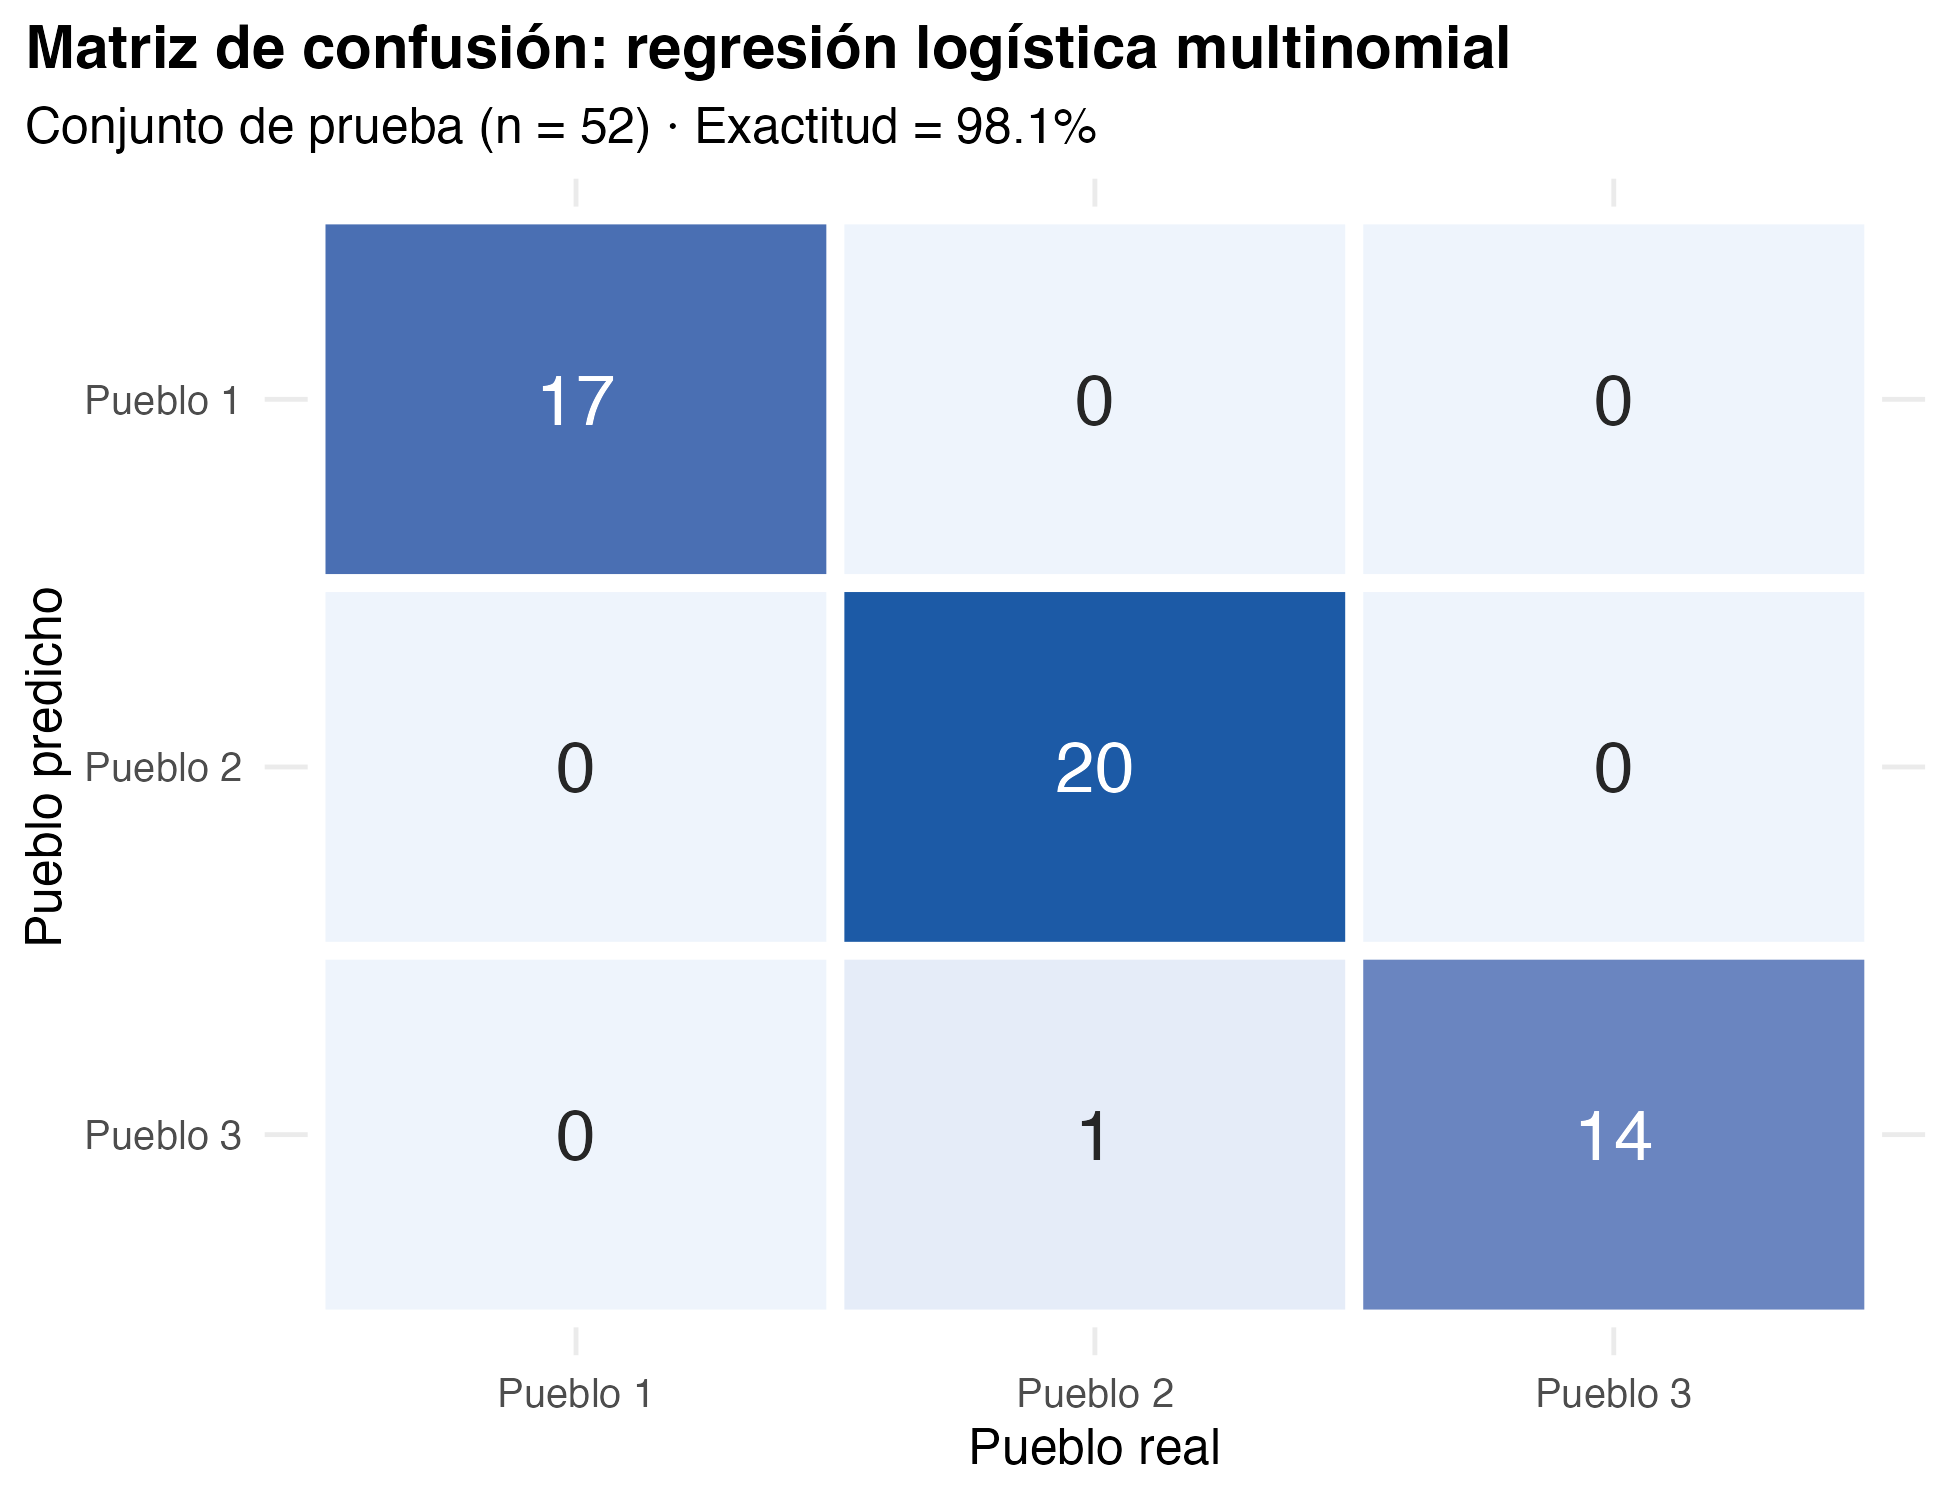
\includegraphics[width=0.88\columnwidth]{07_multinomial_matriz_confusion.png}
  \caption{Matriz de confusión del modelo multinomial en el conjunto de prueba (\textit{n} = 52). La diagonal contiene las muestras clasificadas correctamente; la única muestra mal clasificada es del Pueblo~2 y se predijo como Pueblo~3.}
  \label{fig:confusion}
\end{figure}

\begin{lstlisting}[firstnumber=642]
# Importancia de variables (magnitud de los coeficientes estandarizados, escala 0-100)
imp_pueblo <- varImp(multi_pueblo)$importance %>%
  rownames_to_column("Variable") %>%
  as_tibble() %>%
  rename(Importancia = Overall) %>%
  arrange(desc(Importancia))
imp_pueblo
\end{lstlisting}

La \textbf{importancia de variables} reescala la magnitud de los coeficientes estandarizados de 0 a 100. Los valores más altos fueron \var{Ash\_Alcanity} (100), \var{Proline} (86.3), \var{Color\_Intensity} (84.4) y \var{Flavanoids} (71.1); los más bajos, \var{Nonflavanoid\_Phenols} (0.4) y \var{Magnesium} (0) (Figura~\ref{fig:importancia}).

\begin{figure}[htbp]
  \centering
  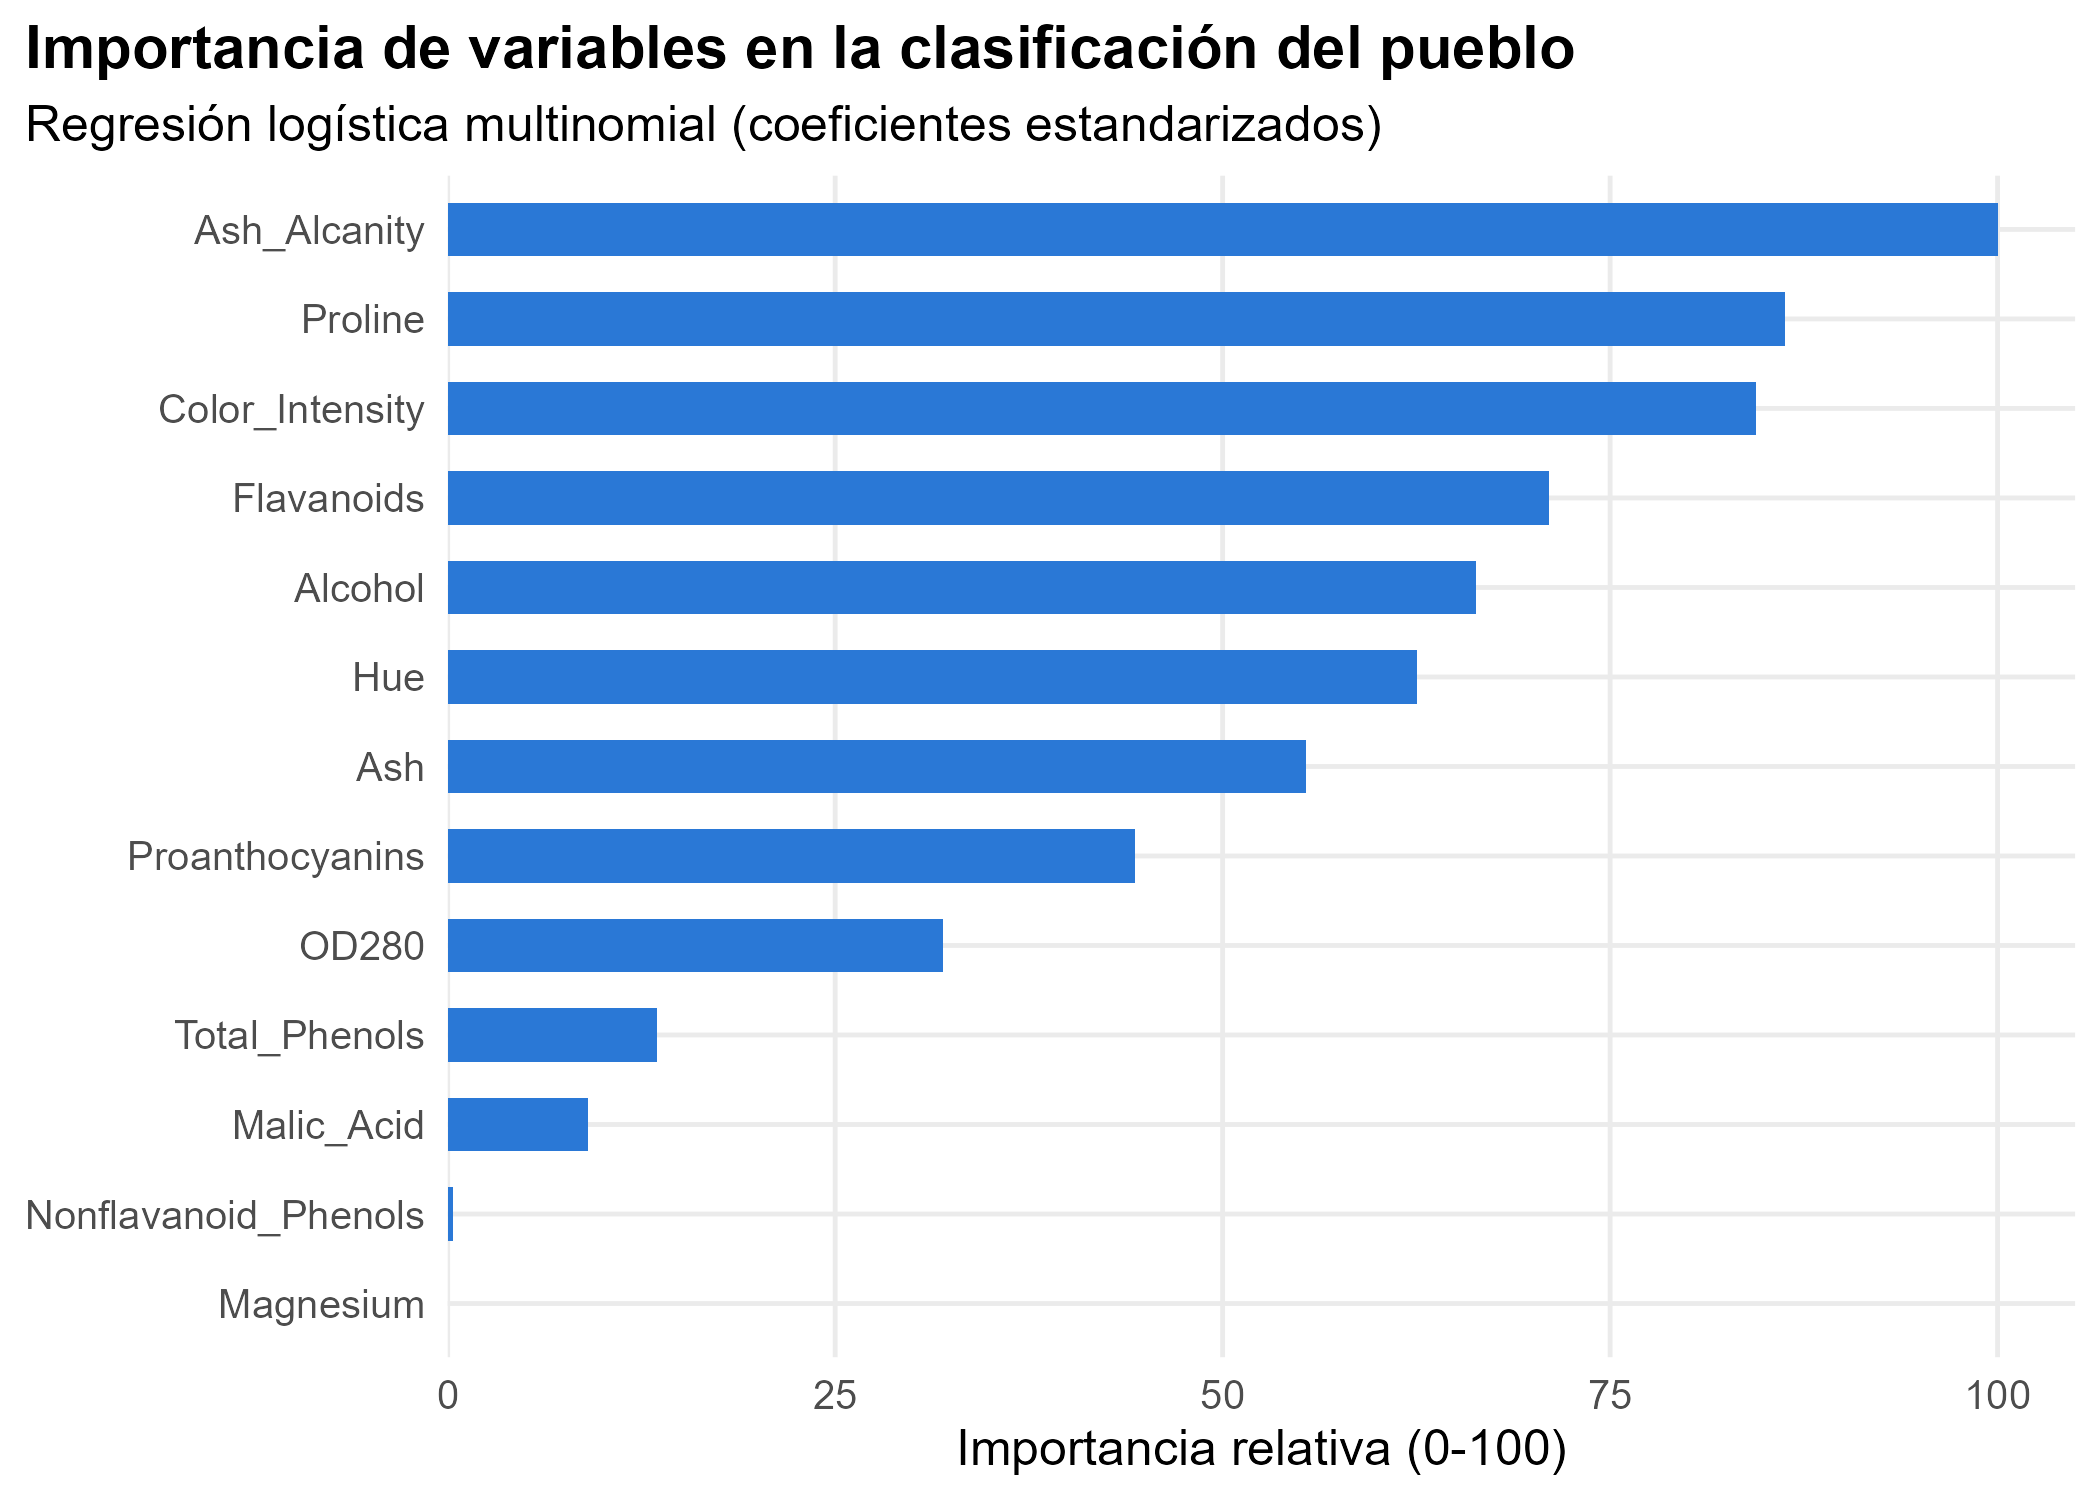
\includegraphics[width=\columnwidth]{08_multinomial_importancia.png}
  \caption{Importancia relativa (0–100) de cada variable en la regresión logística multinomial, calculada a partir de los coeficientes estandarizados.}
  \label{fig:importancia}
\end{figure}

% =======================================================================
\FloatBarrier
\section{Resumen de resultados}

\begin{itemize}
  \item \textbf{Limpieza}: 0 NAs, 0 duplicados y 0 negativos; se corrigió 1 valor con error de formato. La base limpia es de 178 × 14.
  \item \textbf{Exploratorio}: 12 de 13 variables rechazan la normalidad y se detectaron 21 valores atípicos, que se conservaron.
  \item \textbf{3.1}: la prolina difiere entre pueblos (Welch \pval{} = \sci{7.9}{33}; Kruskal-Wallis \pval{} = \sci{1.4}{26}; \etaH{} = 0.669). Las tres comparaciones por pares tienen \pval{} < 0.001.
  \item \textbf{3.2}: las 13 variables difieren entre pueblos (\pval{} ajustado < 0.001). El mayor efecto es el de \var{Flavanoids} (\etaH{} = 0.734) y el menor el de \var{Ash} (0.121).
  \item \textbf{3.3}: 8 variables explican el 63.6\,\% de la variación de la prolina (\textit{R}² ajustado = 0.611). En prueba, RMSE = 210.8 mg/L y \textit{R}² = 0.613, y se cumplen los tres supuestos verificados.
  \item \textbf{3.4}: el modelo multinomial clasifica correctamente 51 de 52 muestras de prueba (exactitud = 0.981, kappa = 0.971).
\end{itemize}

\end{document}
